%\documentstyle[11pt,a4j]{jarticle} 
\documentclass[11pt,a4j]{jarticle}
\usepackage[dvipdfmx]{graphicx}
\usepackage{fancybox}
\usepackage{listings,jlisting}
\usepackage[at]{easylist}
\usepackage{here}
\setlength{\oddsidemargin}{0mm}
\setlength{\textwidth}{170mm}
\setlength{\topmargin}{-5mm}
\setlength{\textheight}{240mm}
\setlength{\columnsep}{8mm}

\setcounter{secnumdepth}{5}
\makeatletter
\newcommand{\subsubsubsection}{\@startsection{paragraph}{4}{\z@}%
    {1.0\Cvs \@plus.5\Cdp \@minus.2\Cdp}%
    {.1\Cvs \@plus.3\Cdp}%
    {\reset@font\normalsize\bf}
}
\newcommand{\subsubsubsubsection}{\@startsection{subparagraph}{5}{\z@}%
    {1.0\Cvs \@plus.5\Cdp \@minus.2\Cdp}%
    {.1\Cvs \@plus.3\Cdp}%
    {\reset@font\normalsize\bf}
}
\makeatother
\setcounter{tocdepth}{5}

\lstset{%
    language={Java},
    basicstyle={\small\ttfamily\footnotesize},%
    identifierstyle={\small},%
    commentstyle={\small\itshape},%
    keywordstyle={\small\bfseries},%
    ndkeywordstyle={\small},%
    stringstyle={\small\ttfamily},
    frame={tb},
    breaklines=true,
    columns=[l]{fullflexible},%
    numbers=left,%
    xrightmargin=0zw,%
    xleftmargin=3zw,%
    numberstyle={\scriptsize},%
    stepnumber=1,
    numbersep=1zw,%
    lineskip=-0.5ex%
}

\begin {document}
\thispagestyle{empty}
\begin{flushright}
    \begin{tabular}{|c|}\hline
        \hspace*{2cm}   \\
        \hspace*{2cm}   \\
        \hspace*{1.7cm} \\ \hline
    \end{tabular}\\
    {\huge\tt 2020-後学期}
\end{flushright}
\begin{center}
    \begin{Huge}
        {\bf 令和2年度 プログラミング演習}\\
        \vspace{0.5cm}
        {\bf グループプログラミング レポート}\\
        \vspace{1.5cm}
        {\bf 「タワーディフェンスゲーム」}\\
        \vspace{5cm}

        \begin{tabular}{|c|c|}\hline
            学科         & 総合情報学専攻 \\ \hline
            クラス       & J1             \\ \hline
            グループ番号 & 1              \\ \hline
            1910002      & 青木 辰磨      \\ \hline
            1910097      & 上田 達也      \\ \hline
            1910110      & 遠藤 誉士      \\ \hline
        \end{tabular}
    \end{Huge}
\end{center}
\newpage

\section{プログラムの概要}
% どの様な目的のプログラムを実現したか,どのような機能を実装したか,
% をまず最初に説明してください.
% 必要に応じてスクリーンキャプチャした画像も張り付けてください.

% 「ドローエディタ」ならば,どのような機能を持ったドローエディタを作ったか
% 説明してください.

% 作業の分担など,作業をどのように進めたかも説明して下さい.


\subsection{目的}

電通大の4Kマップを使ったタワーディフェンスゲームの作成

\subsection{機能}

ゲームは「タイトル・ゲーム・ポーズ・リザルト」の4画面から構成される。

\subsubsection{タイトル画面}

\begin{itemize}
    \item
          ゲーム画面への移行とゲームの終了が出来る。
\end{itemize}

\subsubsection{ゲーム画面}

\begin{itemize}
    \item
          ポーズ画面への移行が出来る。
    \item
          電通大内の主要な建物の内、防衛拠点となるタワーをゲーム毎にランダムに2つ選ぶ。
    \item
          タワーを陥落させるために電通大へと攻めてくる4種類のエネミーと、エネミーを撃退するための3種類のタレットがある。
    \item
          エネミーは、ウェーブ毎にランダムに選出された3つのスポーン地点から出現し、防衛拠点へと侵攻、攻撃する。
    \item
          エネミーの数は、ウェーブ毎に増加する。
    \item
          エネミーを撃退する為に、タレットを購入し、指定されたいくつかの地点に配置できる。
    \item
          タレットは、レベルに応じた金額を支払うことで、「攻撃力・攻撃範囲・攻撃速度」のレベルを上げて強化することが出来る。所持金は、エネミーを撃破することで増やすことが出来る。
    \item
          購入したタレットは、必要に応じて売却することが出来る。売却値はタレットのレベルによって変わる。
    \item
          エネミーがタワーを攻撃し、2つのタワーが陥落したらゲームオーバー。一定のウェーブ数をしのぎ切ればゲームクリアとなる。
    \item
          エネミーの撃破状況とゲームクリア時に残ったタワーの数を参照してスコアを決定する。
\end{itemize}

\subsubsection{ポーズシーン}

\begin{itemize}
    \item
          ゲームの進行を一時停止する。再開時には、ポーズした時点からゲーム画面に移行する。
    \item
          ゲームの再開(ゲーム画面への移行)とゲームの終了(タイトル画面への移行)が出来る。
\end{itemize}

\subsubsection{リザルトシーン}

\begin{itemize}
    \item
          ゲームオーバーとゲームクリアの2種類の画面があり、ゲームのスコアを表示する。
    \item
          タイトル画面への移行が出来る。
\end{itemize}


\subsection{作業分担}

プログラムをMVCモデルに従って構成したため、作業分担も主に「Model・View・Controller」の3つに分けて行った。それとは別に、タワーやエネミー、タレットといった「ゲームオブジェクト」のプログラムをそれぞれが担当した。

以下が、それぞれが担当したプログラムの詳細である。

\begin{itemize}
    \item 上田
          \subitem ゲーム画面のModel
          \subitem タレットが配置可能な場所
          \subitem エネミーの出現
          \subitem マップ製作(タワーやエネミー侵入場所、グラフの頂点の座標を定義)

    \item 遠藤
          \subitem ゲーム画面のView
          \subitem ゲームシステム
          \subitem ゲームオブジェクトの各種エネミー
          \subitem ゲームオブジェクトのタワー
          \subitem スタート、ポーズ、タイトル画面のModel・View・Controller

    \item 青木
          \subitem ゲーム画面のController
          \subitem ゲームオブジェクトの各種タレット
          \subitem エネミーのサーチ(索敵)
          \subitem ゲームサウンド
          \subitem ゲームオブジェクトと各シーンの画像探し
\end{itemize}

始めにゲームシステムの構築を行い、ゲームを作る上で活用する機能を実装した。ゲーム本体のプログラムは、始めにControllerと各ゲームオブジェクトの基盤となるクラスを実装し、実装が出来たものをViewとModelに追加していった。ゲームとして動作するようになった後は、基盤となるクラスを継承した各ゲームオブジェクトを複数種作成し、ゲーム性の拡張とゲームバランスの調整を行った。最後に、スタート、ポーズ、リザルト画面の実装とゲームサウンドの実装を行い、完成へと至った。

プログラムの統合は、Githubを用いて行った。これにより、「誰がどこのプログラムを書いたのか」「どこのプログラムを変更したのか」などの確認が非常にスムーズに出来た。また、万が一途中でプログラムが動かなくなったとしても、直前の状態へと戻すことが出来る為、安心してコードを共有することが出来た。

(文責: 青木)

\section{設計方針}
% プログラムの基本構想を述べる.
% どのようなアルゴリズム,データ構造を用いて,目的の処理を実現するのか説明する.
% なぜ,そのようなアルゴリズム,データ構造を用いたかという考察も含める.
% ここでは,プログラムの細部には触れない.

% 今回は,Javaのプログラミングなので,どのようなクラスを用意して,どのように利用するかを説明する.
% クラス図を使用してください.発表会のプレゼンで作成したクラス図を流用して
% 構いません.

まず、プログラム全体のシーン遷移などを実現するための設計について述べる。

大まかにプログラムはシステム部とシーン部に分けられる。

システム部はウインドウ作成やシーン管理などゲーム内容に関係なく行われる処理を行うクラスと, ベクトルの計算など様々な場面で汎用的に用いるクラスからなる
シーン部はタイトル画面やゲーム画面、ポーズ画面など、場面ごとの動作を記述するクラスからなり、各シーンはシステム部の\verb|Scene|, \verb|SceneModel|, \verb|SceneView|, \verb|SceneController|クラスを継承して作る。

ゲーム内に登場するオブジェクトは基本的にすべてシステム部のクラスの一つである\verb|GameObject|を継承して作る。

シーン部はMVCパターンを用いて構成しており、Modelはデザインパターンの一つであるCompositeパターンを利用して作られたGameObjectの木を持つ。ゲーム内オブジェクトは再帰的な木構造を持つため、これによってゲームに適した粒度にクラスを分割することが可能になり、分担を行うことができた。

システム部とゲーム画面のシーンの関係を示すクラス図を図\ref{fig:Classes}に,ゲームオブジェクトのヒエラルキー図を図\ref{fig:gameSceneHierarchy}に示す.

\begin{figure}[H]
    \begin{center}
        \leavevmode
        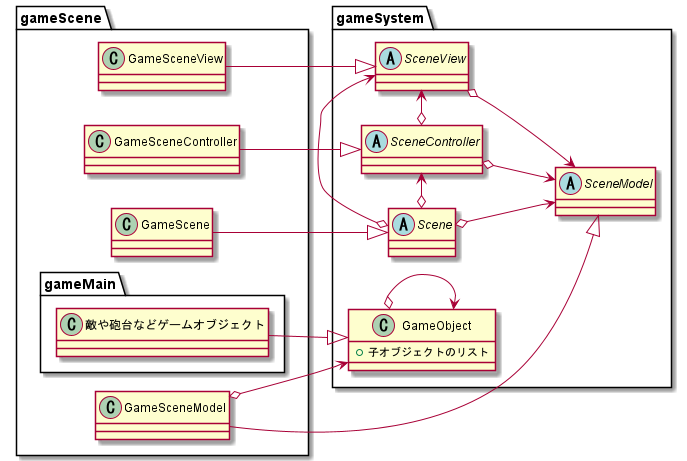
\includegraphics[width=0.9\textwidth]{system.png}
        \caption{システム部クラス図}
        \label{fig:Classes}
    \end{center}
\end{figure}

\begin{figure}[H]
    \begin{center}
        \leavevmode
        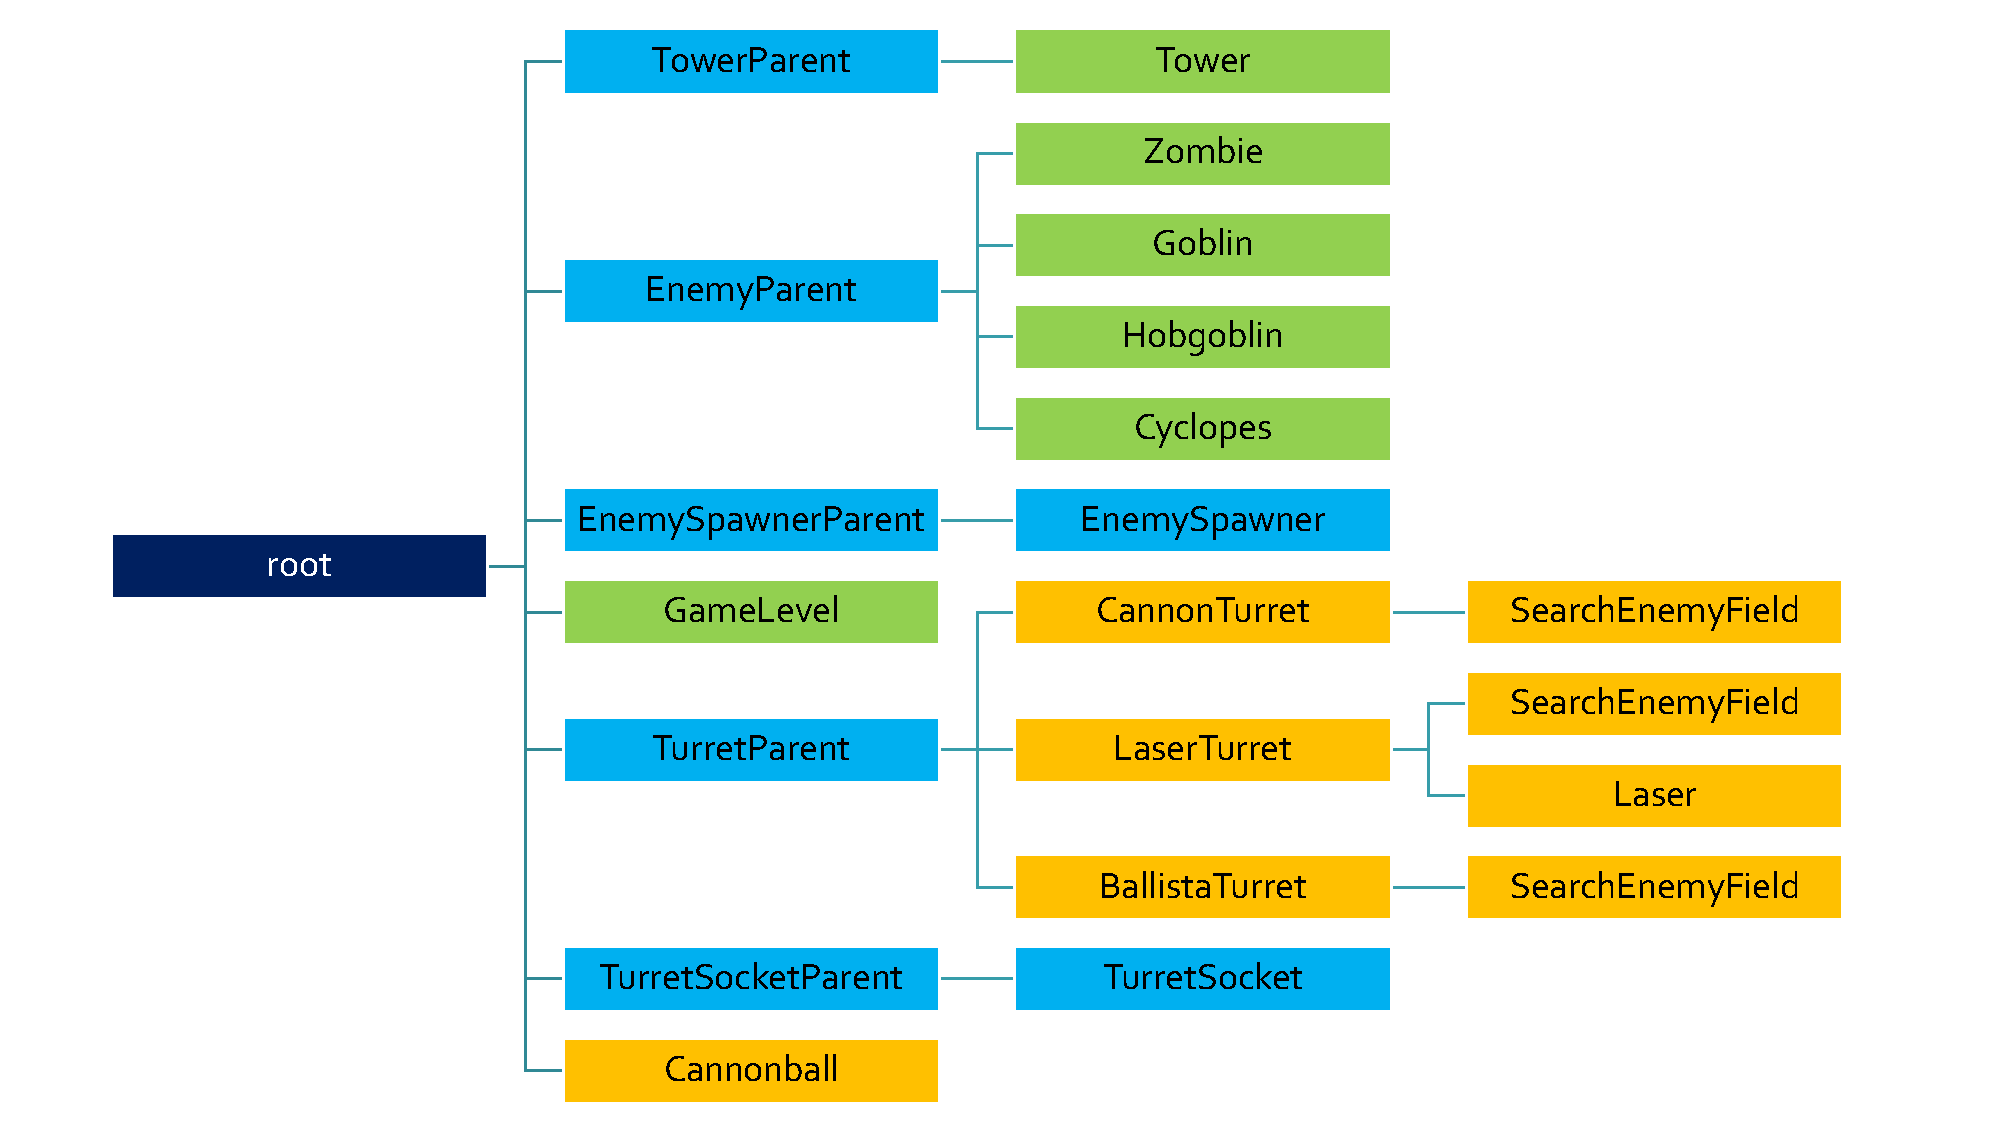
\includegraphics[width=0.9\textwidth]{hierarchy.pdf}
        \caption{ヒエラルキー図例}
        \label{fig:gameSceneHierarchy}
    \end{center}
\end{figure}

\subsection{ゲーム画面}

ゲームを表現するために必要なオブジェクトは、大まかには以下の物がある。

\begin{itemize}
    \item タワー
    \item 敵
          \subitem 敵が移動するための道情報を持つマップ。
    \item タレット
          \subitem 各タレットから発射される砲弾や矢など
\end{itemize}

これらと、ルールの大まかな実装方法について述べる。

\subsubsection{タワー}

タワーを表すクラス\verb|Tower|は、\verb|TowerArranger|クラスによって選出、配置される。また、Towerクラスは攻撃を受けることが可能であることを示すインタフェース\verb|IDamageApplicable|を実装しており、applyDamageメソッドが実行されると攻撃を受ける。耐久値が無くなると陥落し、陥落したことを受け取りたいクラスであることを示す\verb|TowerFallListener|の\verb|onTowerFall|メソッドが実行される。

\subsubsection{敵}

敵は\verb|BaseEnemy|クラスを継承して作られ、ゲーム内では\verb|EnemySpawner|オブジェクトから出現する。\verb|EnemySpawnerManager|はこれを管理するクラスであり、インスタンスの生成、敵の種類や出現間隔、スポナー自体の起動時間などの情報の\verb|EnemySpawner|への入力等を行う。管理のアルゴリズムはStrategyパターンにより柔軟に変えることが変えられるようにした。

敵もタワーと同じく攻撃可能であることを示す\verb|IDamageApplicable|を実装しており、攻撃されると耐久値が減り、無くなると敵が死亡したことを受け取りたいクラスであることを示す\verb|EnemyDieListener|の\verb|onEnemyDead|メソッドが実行される。

敵自体の行動アルゴリズムもStrategyパターンによって変更することが可能になっている。実際に実装されているアルゴリズムは
\begin{itemize}
    \item 襲撃対象をランダムに選択する。
    \item 現在の地点から対象までの最短経路を探索する
    \item これに沿って移動し、対象を攻撃する
    \item 対象が陥落した場合は、別の対象が残っている限り最初から同じことを繰り返す
\end{itemize}
というものである。敵の移動、経路探索等は地図情報を持つオブジェクト\verb|GameLevel|に任せられている。地図情報は\verb|Graph|クラスが持つ。データ構造としては隣接リスト表現でグラフを持っており、頂点情報、辺情報が格納される。
グラフは\verb|GraphBuilder|クラスによって外部ファイルから情報を得て生成される。

\subsubsection{タレット}

タレットは\verb|BaseTurret|クラスを継承して作られる。配置可能な場所を示すオブジェクトである\verb|TurretSocket|がクリックされたときに、購入可能な状態であれば配置される。

配置されたタレット自体を選択することが可能であり、選択されている間は能力の強化、売却ができる。

\subsubsection{ルール}

\verb|GameSceneModel|クラスはゲームの状態、データを管理する。ゲームの主な状態には「次のウェーブを待っている状態」「ウェーブ中」、「ゲームオーバー」、「ゲームクリア」が存在し、時間経過やゲーム内の状態によって遷移する。
また同クラスは\verb|TowerFallListener|, \verb|EnemyDieListener|などのインタフェースを実装し、敵の撃破やタワーの陥落などを監視し、状態遷移やスコアの計算などに使用する。
ゲームオーバー、もしくはクリアの条件を満たしたら一定時間ののち、リザルト画面に遷移する。また、ポーズ入力があった場合、ポーズ画面に遷移する。

(文責: 遠藤)

\section{プログラムの説明}
% メンバー全員が各自の担当した部分を説明.工夫点を述べる.

% 実際に作成した主要なクラスの主なメソッド,フィールドの説明を行う.
% 必要に応じてプログラムリストを抜粋して説明する.

\subsection{遠藤担当分主要クラス}

\subsubsection{MainFrame}

\subsubsubsection{仕様}

static void main()の存在するクラス。JFrameを継承しており、ゲームのメインウインドウとして機能する。また、インタフェースSceneChangeListenerを実装しており、シーン遷移の制御を行う。

\subsubsubsection{フィールド}

\begin{lstlisting}[numbers=none]
private JPanel mainPanel; // 基本的に全てのSwingの要素はこのパネルの下に置く
private CardLayout layout; // カードレイアウトでシーンを切り替える

private Stack<Scene> sceneStack; // シーンを保存しておくスタック
\end{lstlisting}

\subsubsubsection{メソッド}

\subsubsubsubsection{\texttt{createWindows()}}

Swingの機能で新しいウインドウを生成する。

\subsubsubsubsection{\texttt{void sceneChanged(Scene scene, boolean stackClearFlag, Intent intent), sceneChanged(Scene scene, Intent intent)}}

SceneChangeListenerインタフェースのメソッド。

stackClearFlagがTrueならスタックにあるシーンをすべてクリアする。Falseなら一番上にあるシーンをポップして新しいシーンに遷移する。Falseがデフォルト。

\subsubsubsubsection{\texttt{void scenePopped(Intent intent) }}

SceneChangeListenerインタフェースのメソッド。

一番上にあるシーンをポップする。ポーズシーンから戻るときなどに使う。

\subsubsubsubsection{\texttt{void scenePushed(Scene scene, Intent intent)}}

SceneChangeListenerインタフェースのメソッド。

一番上に新しいシーンをプッシュする。ポーズ画面への遷移などに使う。

\subsubsection{Scene}

\subsubsubsection{仕様}

MVC各インスタンスとSceneChangeListenerを持ち、一つのシーンとして機能する。コンストラクタ以外に特にメソッドはない。

\subsubsubsection{フィールド}

\begin{lstlisting}[numbers=none]
protected SceneModel model;
protected SceneView view;
protected SceneController controller;
protected SceneChangeListener sceneChangeListener;
\end{lstlisting}

\subsubsection{SceneModel}

\subsubsubsection{仕様}

MVCのModelを表す基底クラス。

\subsubsubsection{フィールド}

\begin{lstlisting}[numbers=none]
protected SceneChangeListener sceneChangeListener;
protected GameObject rootGameObject;
\end{lstlisting}

\subsubsubsection{メソッド}

抽象クラスのため、ゲームオブジェクトのrootを機能させる処理以外具体的な実装は存在しない。

\subsubsubsubsection{\texttt{start(Intent intent), stop(), pause(), unpause()}}

シーン開始時、終了時、ポーズ時、ポーズ解除時に実行されるメソッド。startは前のシーンから情報を受け取ることができる。

\subsubsubsubsection{\texttt{void addGameObject(GameObject gameObject)}}

rootのゲームオブジェクトの子オブジェクトを追加する処理。

\subsubsection{SceneView}

\subsubsubsection{仕様}

JPanelを継承している、MVCのVを表す基底クラス

\subsubsubsection{フィールド}

\begin{lstlisting}[numbers=none]
protected SceneModel model;
public Camera camera; // カメラを表すGameObject。描画にこのオブジェクトの情報を用いることもできるが、用いないこともできる。
\end{lstlisting}

\subsubsubsection{メソッド}

\subsubsubsubsection{\texttt{start(), stop(), pause(), unpause()}}

シーン開始時、終了時、ポーズ時、ポーズ解除時に実行されるメソッド。

\subsubsubsubsection{\texttt{draw(Graphics g)}}

描画を行うメソッド。paintComponent内で呼び出される。GameObjectのヒエラルキーをDFSして描画できるものだけ取り出し、depthでソートして描画を各オブジェクトにさせる。

\subsubsubsubsection{\texttt{ public Vector2 convertScreenPosToWorldPos(Vector2 screenPos), public Vector2 ConvertWorldPosToScreenPos(Vector2 worldPos) {}}}

カメラの情報から、スクリーン座標とゲーム内の座標(以下ワールド座標とする)を変換するメソッド。

\subsubsection{SceneController}

\subsubsubsection{仕様}

MVCのCを表す基底クラス。javax.swing.timerを用いて短い時間ごとにmodelへの更新処理とviewへの描画処理を通知する。

\subsubsubsection{フィールド}

\begin{lstlisting}[numbers=none]
protected SceneModel model;
protected SceneView view;
protected javax.swing.Timer timer;

private long prevTime = 0; // フレーム時間計算用、前のフレームの時刻
\end{lstlisting}

\subsubsubsection{メソッド}

\subsubsubsubsection{\texttt{start(Intent intent), stop(), pause(), unpause()}}

シーン開始時、終了時、ポーズ時、ポーズ解除時に実行されるメソッド。model,viewに同様のメソッドを実装させる。

\subsubsubsubsection{\texttt{void actionPerformed(ActionEvent e)}}

タイマーから一定時間ごとに呼び出され、modelに更新処理を、viewに描画処理を行わせる。

\subsubsubsubsection{\texttt{IClickable findClickedObject(Vector2 position)}}

このクラスを継承したクラスで使う、クリックされているオブジェクトを探すメソッド。メソッドのないマーカーインタフェースであるIClickableを実装している中で最もdepthが浅いものを探す。

\subsubsection{GameObject}

\subsubsubsection{仕様}

\begin{itemize}
    \item ゲーム内に存在するオブジェクトの基底クラスである
          \subitem ゲーム内に存在するオブジェクトの基底クラスである
    \item ゲーム内での位置を表す座標を持つ
    \item 短い時間ごとに実行される処理、シーン開始時、ポーズ時、ポーズ開始時には各処理が再帰的に呼び出される
    \item オブジェクトが木構造に追加されたとき、削除されたときに処理が呼び出される。この処理が再帰的には呼び出されないのは、システム側がかかわらない状況だからである。
\end{itemize}


\subsubsubsection{フィールド}

\begin{lstlisting}[numbers=none]
protected GameObject root; // 木構造の根のGameObject
public GameObject parent; // 同じく親
public List<GameObject> children; // 同じく子

private boolean enabled; // オブジェクトが有効であることを示すフラグ。有効な時のみ処理が行われる。
public Vector2 position, offset; // オブジェクトの存在する座標の基準点とそこからずれる距離。相対座標を用いて表現した方が適切な場合はoffsetを用いる。
public int depth; // 深さ。Z座標とも言い換えられる。

private List<GameObject> addObjectList, removeObjectList; // 子オブジェクトを追加・削除する時のバッファ

public Collider collider; // 当たり判定
\end{lstlisting}

\subsubsubsection{メソッド}

\subsubsubsubsection{\texttt{start(), \_start(), calc(float deltaTime), \_calc(float deltaTime), pause(), \_pause() unpause(), \_unpause()}}
スタート時、毎フレーム(または十分に短いペース)、ポーズ時、ポーズ解除時に呼び出されるメソッド。
アンダーバー付きのメソッドが内部的には呼び出され、その内部からアンダーバーなしのメソッドが呼び出される。
アンダーバーなしのメソッドはここでは実装が存在しないが、オーバーライドされたときに実装される可能性がある。(必要でないなら実装しないことも可能)

\subsubsubsubsection{\texttt{onSummoned(), onDestroyed()}}
木構造に追加されたとき、削除されたときに呼び出されるメソッド。これもオーバーライドされたときに実装される可能性がある。

\subsubsubsubsection{\texttt{destroy()}}
このオブジェクトを木構造から削除するメソッド。再帰的に子オブジェクトにも適用される。

\subsubsubsubsection{\texttt{addChild(GameObject child), removeChild(GameObject child)}}
子オブジェクトを追加・削除するメソッド。実行した瞬間に処理を行うとデータ構造が破壊されるため、一時的に追加・削除するリストに入れられ、次の\verb|_calc()|実行時に処理される。

\subsubsubsubsection{\texttt{getEnabled(), setEnabled(boolean enabled), onEnabled()}}
オブジェクトが有効であることを示す\verb|enabled|フラグはprivate指定されているため、このゲッター、セッターを通して操作する。
有効になった時にonEnabled()が実行される.

\subsubsubsubsection{\texttt{findChild(Class<G> class\_), findChildFromChildren(Class<G> class\_)}}
子オブジェクトの中である派生クラスに当たるものを探す。
find...From...という名前のものは直接の子だけでなく全ての子孫から再帰的に探す。
該当するもののうち最初に見つけたもののみ返す。

\subsubsubsubsection{\texttt{findChildren(Class<G> class\_), findChildrenFromChildren(Class<G> class\_)}}
前項と同様に子オブジェクトの中である派生クラスに当たるものを探す。
該当するものを全てリスト形式で返す。

例えば\verb|root.findChild(Camera.class)|などとすることでrootの直接の子にCameraクラスが存在すれば探すことができる。

\subsubsubsubsection{\texttt{clone()}}
オブジェクトを複製する際に実行するメソッド。


\subsubsection{GameSceneView}

\subsubsubsection{仕様}

GameSceneModelから情報を受け取り、防衛対象や次のウェーブまでの残り時間など、表示すべき情報を表示する

タレットを強化するためのUIを定義し、表示する

配置するタレットを選択するためのUIを定義し、表示する

\subsubsubsection{フィールド}

\begin{lstlisting}[numbers=none]
private Font font; // UI表示に用いるフォント

private InformationPanel informationPanel; // 情報表示のためのパネル。
public UpgradeTurretPanel upgradeTurretPanel; // 強化対象のタレットとその情報、タレット強化のためのボタンを配置したパネル
public AddTurretPanel addTurretPanel; // 配置するタレットを選択するためのボタンを配置したパネル
private GameSceneModel gSceneModel; // モデルのインスタンス
\end{lstlisting}

いずれのパネルもオブザーバーパターンを用いてModelから情報の変化を受け取り、表示する情報を変更する。

\subsubsubsubsection{\texttt{InfomationPanel}}

\begin{itemize}
    \item 次のウェーブ開始までの秒数
    \item 現在のウェーブ数
    \item 所持金
    \item 防衛対象
\end{itemize}

を表示するパネル。GridBagLayoutを使用している。

\subsubsubsubsection{\texttt{UpgradeTurretPanel}}

\begin{itemize}
    \item 現在強化対象になっているタレットの画像と名前
    \item 現在の強化対象の範囲レベル、連射速度レベル、威力レベルの表示
    \item 現在の強化対象の範囲強化、連射速度強化、威力強化ボタンの配置
\end{itemize}

を行うパネル。これもGridBagLayoutを使用している

\subsubsubsubsection{\texttt{AddTurretPanel}}

配置するタレットの種類を選択するためのボタンを配置するパネル。

\subsubsubsection{メソッド}

\subsubsubsubsection{\texttt{update(Observable o, Object arg)}}

Java標準のObservableクラスを継承したクラスからゲームのウェーブ数を受け取り、それによってBGMを変える。

\subsubsection{BaseEnemy}

\subsubsubsection{仕様}

このクラスを継承して敵クラスを作成する。基本的に敵としての行動のほとんどの処理はBaseEnemyActStrategyクラスに委譲する。

耐久値などのパラメータと行動パターンさえ渡せば簡単に敵の種類を増やせるようにしている。

\subsubsubsection{フィールド}

\begin{lstlisting}[numbers=none]
// 耐久、攻撃、スピード、ドロップ金額
protected double hp, attackPower, speed;
protected int dropValue;

protected BaseEnemyActStrategy mover; // Strategyパターンを使用して実装、敵の行動パターンを表すクラス
protected GameLevel level; // ゲームのマップデータのオブジェクト。経路探索に使う
protected ArrayList<Tower> targets; // 襲撃対象のリスト
protected Graph.Vertex initialVertex; // 最初に出現したマップ上の地点

protected ArrayList<EnemyDieListener> enemyDieListeners; // この敵が撃破されたときの通知を受け取るリスナーの一覧
\end{lstlisting}

\subsubsubsection{主なメソッド}

\subsubsubsubsection{\texttt{getHp(), getAttackPower(), getSpeed(), getDropValue(), getDropScore(), getInitialVertex()}}

体力、攻撃力、スピード、撃破時の賞金、撃破時のスコア、初期地点のゲッター

\subsubsubsubsection{\texttt{calc(), onSummoned(), onDestroyed()}}

GameObjectに存在するメソッドをオーバーライドして、行動パターンのクラスに委譲している。

\subsubsubsubsection{\texttt{addEnemyDieListener(EnemyDieListener enemyDieListener) , removeEnemyDieListener(EnemyDieListener enemyDieListener) }}

敵撃破時のイベントを受け取るリスナーの登録、解除

\begin{lstlisting}[numbers=none]
public double getHp() {}
public double getAttackPower() {}
public double getSpeed() {}
public int getDropValue() {}
@Override
public void calc(float deltaTime) {}
@Override
public void applyDamage(Damage d) {}
public void addEnemyDieListener(EnemyDieListener enemyDieListener) {}
public void removeEnemyDieListener(EnemyDieListener enemyDieListener) {}
public Graph.Vertex getInitialVertex() {}
\end{lstlisting}

\subsubsection{Graph}

\subsubsubsection{仕様}

マップのデータを表すデータ構造としての役割を持つクラス。重み付き無向グラフを隣接リスト表現で持ち、各頂点は座標や固有の識別番号などの情報を持つ。辺はどの識別番号の頂点からどの頂点へ行くのかという情報、距離を持つ。

\subsubsubsection{フィールド}

\begin{lstlisting}[numbers=none]
public ArrayList<Vertex> vertexes; // 頂点の情報のリスト
public ArrayList<ArrayList<Edge>> data; // 隣接リスト表現のマップデータ
\end{lstlisting}

\subsubsubsection{メソッド}

\subsubsubsubsection{\texttt{addVertex(Vector2 position, int idx)}}

座標と固有の番号を指定して頂点を追加する。

\subsubsubsubsection{\texttt{addEdge(int from, int to)}}

2頂点の番号から辺を追加する。距離はそれぞれの頂点の座標から求める。

\subsubsubsubsection{\texttt{newarestVertex(Vector2 position)}}

ある座標に最も近い頂点を返す。

\subsubsubsubsection{\texttt{Stack<Vertex> shortestPath(Vertex s, Vertex t)}}

ある頂点からある頂点までの最短経路をたどるのに必要な頂点をスタックに入れて返す。具体的な実装は二分ヒープを用いたDijkstra法。

(文責: 遠藤)

\subsection{上田担当分主要クラス}

\subsubsection{GameSceneModel}

\subsubsubsection{仕様}

\begin{easylist}[itemize]
    @ Controllerが操作を受け取り、Modelに反映できるような機能を持つ
    @@ カメラの移動と拡縮
    @@ マウス操作

    @ ゲームの状態遷移を行う
    @@ ゲームクリア・ゲームオーバーのチェック
    @@ タイマーによる制御
    @@ 遷移時の処理
\end{easylist}

\subsubsubsection{フィールド}

\begin{lstlisting}[numbers=none]
private final float cameraZoomSpeed = 0.3f; // カメラの拡縮スピード
private final float cameraZoomMax = 2.0f; // カメラ拡大の最大値
private final float cameraZoomMin = 0.2f; // カメラ縮小の最小値
private BackGround backGround; // 背景
private Camera camera;
private Vector2 cameraMoveDirection; // 正規化された、カメラが動くベクトルが入る変数
private double cameraSpeed; // カメラの移動速度に緩急をつけるための変数
private int cameraZoomOperation; // カメラの拡縮操作をControllerから受け取るための変数。範囲[-1,1]の整数が格納される。
private GameTimer nextWaveTimer, waveEndTimer, gameOverTimer, gameClearTimer;
// 次waveを待機するためのタイマー、wave開始から終了までのタイマー、ゲームオーバーとゲームクリア遷移まで待機するためのタイマー
public ObservableComponent<GameState> currentState; // 現在のGameState
public ObservableComponent<Integer> countdownNum, waveNum, numOfEnemies, balance, maxWaveNum, score;
// wave開始前のカウントダウン値、現在ウェーブ数、マップ上の敵数、所持金、最大ウェーブ数(このウェーブを凌げばクリア)、スコア
public ObservableComponent<ArrayList<BaseTurret>> availableTurretList; // 利用可能なタレット群
public ObservableComponent<BaseTurret> selectingTurret; // 画面右にタレット情報を表示させるための変数
public ObservableComponent<BaseTurret> purchasingTurret; // 購入対象のタレット
private EnemySpawnerManager enemySpawnerManager; // waveごとにEnemySpawnerを配置するためのクラス
public ObservableComponent<ArrayList<Tower>> targets; // 襲撃目標群
// 新しく作成されるゲーム内オブジェクトが属する、ゲーム内オブジェクトのヒエラルキーの親
private TurretParent turretParent; // タレットの親クラス
private TowerParent towerParent; // タワーの親クラス
private EnemySpawnerParent enemySpawnerParent; // スポナーの親クラス
\end{lstlisting}

\subsubsubsection{メソッド}

\subsubsubsubsection{\texttt{receiveIClickable(IClickable iClickable)}}

Controllerが、クリックされたIClickableのオブジェクトをModelに通知するためのメソッド。受け取るオブジェクトのクラスによって処理が以下のように変わる。

\begin{easylist}[itemize]
    @ nullである場合
    @@ 選択中のタレットをnullにする
    @ BaseTurretのインスタンスである場合
    @@ 選択中のタレットをクリックされたタレットに更新する
    @ TurretSocketのインスタンスである場合
    @@ 選択中のタレットがnullでなければ、そのTurretSocketに対しタレットの設置を試みる
\end{easylist}

\subsubsubsubsection{\texttt{setCameraMoveDirection(Vector2 cameraMoveDirection)}}

Controllerが、キー入力を受け取りカメラ移動ベクトルを計算し、そのベクトルをModelに渡すためのメソッド。

\subsubsubsubsection{\texttt{setCameraZoomOperation(int cameraZoomOperation)}}

Controllerが、キー入力を受け取りカメラの拡縮操作を範囲[-1,1]の整数に変換し、Modelに渡すためのメソッド。

\subsubsubsubsection{\texttt{actionPerformed(ActionEvent e)}}

タイマーから呼び出されることで、ゲームの状態遷移を行うメソッド。ActionEventとして受け取るタイマーの種類により処理が以下のように変わる。

\begin{easylist}[itemize]
    @ nextWaveTimerの場合
    @@ カウントダウン値を減らしながらwave開始までのカウントダウンを行う。
    @@ カウントダウンが終了したらcurrentStateをOnWaveとし、waveEndTimerを起動する。
    @ waveEndTimerの場合
    @@ waveNumがmaxWaveNumに一致しない、すなわち凌ぎ切ればクリアとなるウェーブ数に満たない場合は、currentStateをWaitingForNextWaveとし、カウントダウン値を初期化し、nextWaveTimerを起動する。
    @@ waveNumがmaxWaveNumに一致する場合はゲームクリアとなる。リザルト画面遷移までのタイマーであるgameClearTimerを起動させる。
    @ gameOverTimerおよびgameClearTimerの場合
    @@ スコアを計算し、Intentとしてスコアとクリアの成否の情報をResultSceneに渡す。ResultSceneに遷移する。
\end{easylist}

\subsubsubsubsection{\texttt{calc(float deltaTime)}}

フレーム毎に必要となる処理を記述するメソッド。本プログラムではカメラの移動と拡縮を行う。カメラ操作の入力はControllerが受け取り、移動方向ベクトルと拡縮操作を範囲[-1,1]の整数で表したものをModelに渡す。これらはそれぞれModelのフィールドであるcameraMoveDirectionとcameraZoomOperationに格納される。よって、calcメソッドでそれらの値を元にカメラをマイフレーム毎に操作することで、カメラの移動と拡縮を実装している。

\subsubsubsubsection{\texttt{onTowerFall(Tower tower)}}

襲撃目標が破壊されたときに呼ばれるメソッド。全目標が破壊された場合、currentStateがGameClearでなければゲームオーバーのリザルトシーンに遷移するための処理を行う。currentStateをGameOverにし、gameOverTimerを起動させる。クリア条件は「maxWaveNumのウェーブを凌ぎ切った時点でクリア」であるため、クリア後にゲームオーバーの判定を行わないようにした。

\subsubsubsubsection{\texttt{pauseKeyPressed()}}

ポーズキーの入力時にControllerから呼ばれるメソッド。ポーズ中のシーンに遷移する。

\subsubsection{EnemySpawner}

\subsubsubsection{仕様}

\begin{easylist}[itemize]
    @ ゲーム内オブジェクトクラスGameObjectを継承する
    @ マップに設置されると、敵を自分の場所に一定時間間隔で出現させる
    @ 一定の敵数が出現したら出現を止める
    @ ゲームのポーズ時にタイマーを止め、再開時に戻すことができる
\end{easylist}

\subsubsubsection{フィールド}

\begin{lstlisting}[numbers=none]
private int spawnCount; // 敵出現数。
private int initialDelay; // Wave開始から敵出現開始までの遅延(ms)
private int spawnDelay; // 敵出現間隔(ms)
private GameTimer timer; // 出現待ちに用いるゲーム内タイマー
private BaseEnemy spawnEnemy; // 出現敵種
private Vertex initialVertex; // 敵出現地点
private EnemyParent enemyParent; // 出現した敵が属するゲーム内オブジェクトのヒエラルキーの親
private EnemyDieListener enemyDieListener; // エネミー死亡リスナー
\end{lstlisting}

\subsubsubsection{メソッド}

\subsubsubsubsection{\texttt{actionPerformed(ActionEvent e)}}

spawnCountが0より大きいならば、敵を自身の場所に出現させ、spawnCountを1減らす。タイマーがspawnDelayのミリ秒分の周期でactionPerformedを呼び出す。

\subsubsubsubsection{\texttt{public void pause(), public void unpause()}}

ゲームをポーズする際にEnemySpawnerが停止しなければ、ポーズ画面の裏で敵が出現し続けることになる。よって、EnemySpawnerがフィールドに持つタイマーを停止および再開することが出来るメソッドとしてこれらを定義した。

\subsubsection{TurretSocket}

\subsubsubsection{仕様}

\begin{easylist}[itemize]
    @ タレットの土台の役割を持つ。よって、タレットを持つことができる。
    @ 設置処理はModelが行うため、TurretSocketでは実装しない。その代わり、Modelからタレット配置処理を呼び出せるようパブリックメソッドtryBuildTurretを用意する。
    @ IClickableをimplementsする。Controllerはクリックされたオブジェクト(IClickable)を検索してModelに渡すことができ、これを用いるため。
\end{easylist}

\subsubsubsection{フィールド}

\begin{lstlisting}[numbers=none]
private TurretParent turretParent; // 配置されたタレットが属するゲーム内オブジェクトのヒエラルキーの親
private BaseTurret turret; // タレットを持つ。配置されていない間はnullとする
\end{lstlisting}

\subsubsubsection{メソッド}

\subsubsubsubsection{\texttt{tryBuildTurret(BaseTurret turret)}}

Modelは、TurretSocketがクリックされると、そのTurretSocketに対しtryBuildTurretを呼び出す。この際、引数には選択中のタレットが入る。こうすることで、タレットが選択された状態でTurretSocketをクリックすると、そのTurretSocketに選択中のタレットを建設できる。

「タレットの設置を試みる」とした理由は二つある。まず一つ目に、タレットが選択中でない場合は、選択中のタレットがnullとなるためである。二つ目は、TurretSocketにすでにタレットが設置されている場合は設置処理をしないためである。

\subsubsection{TurretSocketArranger}

\subsubsubsection{仕様}

TurretSocketを配置する機能を持ったクラスであり、フィールド変数はない。

\subsubsubsection{メソッド}

\subsubsubsubsection{\texttt{arrangeTurrets(String turretSocketsPath, GameObject root, TurretSocketParent turretSocketParent,TurretParent turretParent)}}

Scannerを用いて、TurretSocketを配置する座標を記述したファイルを読み込み、マップ上に配置する。ファイルのフォーマットは一行目が入力行数、それ以降がTurretSocketを配置するマップ上のx座標とy座標となっている。

(文責: 上田)

\subsection{青木担当分主要クラス}
\subsubsection{GameSceneController}
\begin{description}
    \item[仕様]\mbox{}\\
          マウスやキーの操作を受け取り、その際の動作をGameSceneModelに渡す
          \begin{itemize}
              \item 画面の移動(WASDキー)
              \item 画面の拡縮(Shift Spaceキー)
              \item タレットの配置と売却とアップデート(マウスの左クリック)
          \end{itemize}
    \item[フィールド]\mbox{}\\
          \begin{lstlisting}[numbers=none]
            private boolean isWKeyPressed;
            private boolean isAKeyPressed;
            private boolean isSKeyPressed;
            private boolean isDKeyPressed;
            private boolean isSHIFTKeyPressed;
            private boolean isSPACEKeyPressed;
            // WASD及びShift, Spaceキーが押されているかを判定するフィールド(押されていればtrue、押されていなければfalseとなる)

            private GameSceneModel gameModel;
            private GameSceneView gameView;
            // GameSceneModelとGameSceneViewを表すフィールド

            private GameSceneView.AddTurretPanel addTurretPanel;
            private GameSceneView.UpgradeTurretPanel upgradeTurretPanel;
            // タレット購入ボタンがあるパネルとアップグレードボタンがあるパネルを表すフィールド

            private JButton rangeButton, powerButton, rofButton, sellButton;
            // タレットのアップグレードと売却をするボタンを表すフィールド

            private ObservableComponent<ArrayList<TurretDisplayButton>> turretButtons;
            // タレットの購入ボタンを要素とする配列を表すフィールド
                \end{lstlisting}
    \item[メソッド]\mbox{}\\
          \begin{description}
              \item[public void actionPerformed(ActionEvent e)]\mbox{}\\
                    各ボタンからのイベントを受け取った際に、GameSceneModelでタレットの購入や売却、アップデートを行うメソッド。
              \item[public void addActionListenerToTurretButtons()]\mbox{}\\
                    タレットボタンにActionListenerを付与するフィールド。
              \item[public void moveCamera()]\mbox{}\\
                    画面の移動を行うメソッド 。WASDキーが押されているかどうかによって方向ベクトルを求め、それを標準化してGameSceneModelに渡している。
              \item[public void updateScaleOperation()]\mbox{}\\
                    画面の拡縮を行うメソッド 。Shift, Spaceキーが押されているかどうかによって拡縮を判断し、それをGameSceneModelに渡している。
              \item[public void mouseClicked(MouseEvent e)] \mbox{}\\
                    マウスで左クリックした座標をGameSceneModelに渡すメソッド。クリックした座標を受け取ったら、その座標をワールド座標に変換してから、クリック可能なゲームオブジェクトをクリックしているかどうかを確かめる。もしクリックしていたらmodelにそれを通知。クリックしていなかったらNULLを返す。クリックしているオブジェクトは、findClickedObjectにワールド座標を渡して判断する。
              \item[public void keyPressed(KeyEvent e)] \mbox{}\\
                    キーを押した時、それが特定のキー(WASD, Shift, Spaceキー)ならば、それぞれの判定フィールドをtrueにする。また、WASDキーを押した時にはmoveCameraメソッドを、ShiftまたはSpaceキーを押した時にはupdateScaleOperationメソッドをそれぞれ呼び出す。
              \item[public void keyReleased(KeyEvent e)] \mbox{}\\
                    キーを離した時、それが特定のキー(WASD, Shift, Spaceキー)ならば、それぞれの判定フィールドをfalseにする。また、WASDキーを押した時にはmoveCameraメソッドを、ShiftまたはSpaceキーを押した時にはupdateScaleOperationメソッドをそれぞれ呼び出す。
              \item[public void update(Observable o, Object arg)] \mbox{}\\
                    turretButtonsの変更を検知すると、その変更をaddActionListenerToTurretButtonsフィールドに伝えるフィールド。
          \end{description}
\end{description}

\subsubsection{BaseTurret}
\begin{description}
    \item[仕様]\mbox{}\\
          全タレットの親クラスであり、タレットの持つ情報を外部へと渡したり、パラメータのレベルアップを行うクラス。タレットの持つ情報は以下のようなものがある。
          \begin{itemize}
              \item 名前
              \item 画像
              \item 攻撃力とそのレベル
              \item 攻撃範囲とそのレベル
              \item 攻撃速度とそのレベル
              \item 最大レベル
              \item 購入金額
              \item 売却金額
          \end{itemize}
    \item[フィールド]\mbox{}\\
          \begin{lstlisting}[numbers=none]
protected String name; //名前のフィールド
protected double turretCollisionRadius; //攻撃範囲のフィールド
protected double attackPower; //攻撃力のフィールド
protected int rof; //攻撃速度のフィールド
protected int attackLevel; //攻撃力のレベルのフィールド
protected int rangeLevel; //攻撃範囲のレベルのフィールド
protected int rofLevel; //攻撃速度のレベルのフィールド
protected int maxLevel; //各パラメータの最大レベル(共通)のフィールド
protected int purchasePrice; //購入金額のフィールド
protected Image[] images; //画像のフィールド
protected IMoneyTransfer iMoneyTransfer;  //所持金を追加するフィールド
protected GameObject enemyParentObject; //エネミーの親クラスのフィールド
\end{lstlisting}
    \item[メソッド]\mbox{}\\
          \begin{description}
              \item[protected void onSummoned()]\mbox{}\\
                    タレットを配置した時に処理を行うメソッド。ここでは、エネミーの親クラスを機構造の中から探している。
              \item[public void sell()]\mbox{}\\
                    タレットを売却する処理を行うメソッド。implementしたiMoneyTransferを利用して、タレット売却時にタレットの売却値分だけ所持金が増えるようにしている。
              \item[public double getTurretCollisionRadius()]\mbox{}\\
                    攻撃範囲(turretCollisionRadius)を外部に渡すメソッド。
              \item[public double getAttackPower()]\mbox{}\\
                    攻撃力(attackPower)を外部に渡すメソッド。
              \item[public int getRof()] \mbox{}\\
                    攻撃速度(rof)を外部に渡すメソッド。
              \item[public Image getImage()] \mbox{}\\
                    タレットの画像(image)を外部に渡すメソッド。
              \item[public String getName()] \mbox{}\\
                    タレットの名前(name)を外部に渡すメソッド。
              \item[public int getAttackLevel()] \mbox{}\\
                    攻撃力のレベル(attackLevel)を外部に渡すメソッド。
              \item[public int getRangeLevel()] \mbox{}\\
                    攻撃範囲のレベル(rangeLevel)を外部に渡すメソッド。
              \item[public int getRofLevel()]\mbox{}\\
                    攻撃速度のレベル(rofLevel)を外部に渡すメソッド。
              \item[public int getMaxLevel()]\mbox{}\\
                    各パラメータの最大レベル(maxLevel)を外部に渡すメソッド。
              \item[public abstract int getSalePrice()]\mbox{}\\
                    売却金額を外部に渡すメソッド。売却金額の計算は他のクラスで行うため、抽象クラスとなっている。
              \item[public int getPurchasePrice()]\mbox{}\\
                    購入金額(purchasePrice)を外部に渡すメソッド。
              \item[public abstract int getAttackPowerLevelupPrice()]\mbox{}\\
                    攻撃力をレベルアップした時に上がった売却金額を外部に渡すメソッド。売却金額の計算は他のクラスで行うため、抽象クラスとなっている。
              \item[public abstract int getTurretCollisionRadiusLevelupPrice()]\mbox{}\\
                    攻撃範囲をレベルアップした時に上がった売却金額を外部に渡すメソッド。売却金額の計算は他のクラスで行うため、抽象クラスとなっている。
              \item[public abstract int getRofLevelupPrice()]\mbox{}\\
                    攻撃速度をレベルアップした時に上がった売却金額を外部に渡すメソッド。売却金額の計算は他のクラスで行うため、抽象クラスとなっている。
              \item[public void onSelected()]\mbox{}\\
                    対象を選択している時に処理を行うメソッド。
              \item[public void onUnSelected()]\mbox{}\\
                    対象を選択していない時に処理を行うメソッド。
              \item[public void upAttackLevel()]\mbox{}\\
                    攻撃力のレベルアップの処理を行うメソッド。
              \item[public void upRangeLevel()]\mbox{}\\
                    攻撃範囲のレベルアップの処理を行うメソッド。
              \item[public void upRofLevel()]\mbox{}\\
                    攻撃速度のレベルアップの処理を行うメソッド。
              \item[public BaseTurret clone()]\mbox{}\\
                    タレットの複製を行うメソッド。これにより、タレットを新しく配置する度にBaseTurretを作る必要がない。
          \end{description}
\end{description}

\subsubsection{LaserTurret}
\begin{description}
    \item[仕様]\mbox{}\\
          レーザー塔の処理を行うクラスであり、エネミーにレーザーで攻撃を行う処理や、レベルに応じた各パラメータの計算を行う。
    \item[フィールド]\mbox{}\\
          \begin{lstlisting}[numbers=none]
    private static final double TURRET_RADIUS = 50; // 見た目の大きさを表す定数フィールド。
    private int attackPowerLevelupPrice; //攻撃力をレベルアップした時に上がった売却金額を表すフィールド。
    private int turretCollisionRadiusLevelupPrice; //攻撃範囲をレベルアップした時に上がった売却金額を表すフィールド。
    private int rofLevelupPrice; //攻撃速度をレベルアップした時に上がった売却金額を表すフィールド。
    private int totalPurchasePrice = 0; //タレットの購入とレベルアップで払った金額の合計を表すフィールド。売却金額の計算に用いる。
    ArrayList<GameObject> nearEnemies; //レーザー塔の攻撃範囲内にいるすべてのエネミーを表す配列フィールド。
    private final static double LEVELUP_ATTACK_POWER = 0.2; //攻撃力のレベルアップの計算式に用いる比例定数のフィールド。
    private final static double LEVELUP_COLLISION_RADIUS = 10; //攻撃範囲のレベルアップの計算式に用いる比例定数のフィールド。
    private final static double INTERCEPT_COLLISION_RADIUS = 150; //初期レベル(レベル1)時の攻撃範囲を表す比例フィールド。
    private final static int LEVELUP_LANDING_TIME = 50; //攻撃速度のレベルアップの計算式に用いる比例定数のフィールド。
    private final static int LEVELUP_PRICE = 10; //レベルアップした際の売却金額の計算式に用いる比例定数のフィールド。
    private static final double INTERCEPT_ATTACK_POWER = 1; //初期レベル(レベル1)時の攻撃力を表す比例フィールド。
    private SearchEnemyField searchEnemyField; //一定範囲内のエネミーを探す円形のオブジェクトを表すフィールド。
    private GameTimer timer; //ゲームタイマーを表すフィールド。
                \end{lstlisting}
    \item[メソッド]\mbox{}\\
          \begin{description}
              \item[public void onDestroyed()]\mbox{}\\
                    レーザー塔が削除(売却)された時に処理を行うメソッド。ゲームタイマーを停止する。
              \item[protected void onSummoned()]\mbox{}\\
                    レーザー塔を配置した時に処理を行うメソッド。索敵範囲をセットしたsearchEnemyFieldを木構造における自身の子に加えて、ゲームタイマーをスタートする。
              \item[public void upAttackLevel()]\mbox{}\\
                    レベルアップにより上昇した攻撃力の計算を行うメソッド。計算式は「初期レベルの攻撃力 + 比例定数 * 攻撃力のレベル」である。また、Laserクラスに攻撃力の値を渡している。
              \item[public void upRangeLevel()]\mbox{}\\
                    レベルアップにより上昇した攻撃範囲の計算を行うメソッド。計算式は「初期レベルの攻撃範囲 + 比例定数 * 攻撃範囲のレベル」である。また、Laserクラスに攻撃範囲の値を渡している。
              \item[public void upRofLevel()] \mbox{}\\
                    レベルアップにより上昇した攻撃速度の計算を行うメソッド。計算式は「初期レベルの攻撃速度 - 比例定数 * 攻撃速度のレベル」である。ここでは、ゲームタイマーを一度停止し、新たに計算した攻撃速度(rof)をゲームタイマーに渡して、再度タイマーをスタートすることで、攻撃速度の変化を実現している。
              \item[public int getAttackPowerLevelupPrice()] \mbox{}\\
                    攻撃力をレベルアップした時に上がった売却金額を外部に渡すメソッド。計算式は「初期レベルの売却値 + 比例定数 * 攻撃力のレベル」である。
              \item[public int getTurretCollisionRadiusLevelupPrice()] \mbox{}\\
                    攻撃範囲をレベルアップした時に上がった売却金額を外部に渡すメソッド。計算式は「初期レベルの売却値 + 比例定数 * 攻撃範囲のレベル」である。
              \item[public int getRofLevelupPrice()] \mbox{}\\
                    攻撃速度をレベルアップした時に上がった売却金額を外部に渡すメソッド。計算式は「初期レベルの売却値 + 比例定数 * 攻撃速度のレベル」である。
              \item[public int getSalePrice()] \mbox{}\\
                    売却金額を計算して外部に渡すメソッド。計算式は「(購入金額 + レーザー塔に使った金額の合計) * 0.8」である。
              \item[public void hitLaser()] \mbox{}\\
                    レーザーを発射するメソッド。攻撃範囲内にいる攻撃済みのエネミーを集合enemySetInAttackに加え、攻撃範囲内のエネミーがenemySetInAttackに含まれていなければ、Laserクラスを作って攻撃を行う。これにより、一度攻撃したエネミーに対してLaserを生成し続けてゲームの処理が重くなってしまうのを防いだ。また、Laserクラスを生成した際に、Laserクラスを自身の子に加えている。
              \item[public void actionPerformed(ActionEvent e)] \mbox{}\\
                    ゲームタイマーが動いている時に、hitLaserメソッドを呼び出すメソッド。
              \item[public void pause()] \mbox{}\\
                    ポーズした時の処理を行うメソッド。タイマーを一時停止する。
              \item[public void unpause()] \mbox{}\\
                    ポーズを解除した時の処理を行うメソッド。タイマーを再開する。
              \item[public void onSelected()] \mbox{}\\
                    レーザー塔を選択している時に処理を行うメソッド。searchEnemyFieldを表示する為にフラグをtrueにする。
              \item[public void onUnSelected()] \mbox{}\\
                    レーザー塔を選択していない時に処理を行うメソッド。searchEnemyFieldを表示しない為にフラグをfalseにする。

          \end{description}
\end{description}


\subsubsection{Laser}
\begin{description}
    \item[仕様]\mbox{}\\
          レーザー塔から発射されるレーザーの処理を行うクラスであり、レーザーの表示やエネミーにダメージを与える処理を行う。
    \item[フィールド]\mbox{}\\
          \begin{lstlisting}[caption=uectd.game.gameScene.gameMain,label=Laser, numbers=none]
            protected double attackPower; //攻撃力を表すフィールド
            protected double radius; //円形の攻撃範囲の半径を表すフィールド
            private IAttackable attacker; //攻撃するタレット(レーザー塔)を表すフィールド
            private GameObject enemyParentObject; //エネミーの基底クラスを表すフィールド
            protected BaseEnemy nearEnemy; //攻撃範囲内にいるエネミーの内の1体を表すフィールド
            private GameTimer timer; //ゲームタイマーを表すフィールド
            private Image image; //レーザーの画像を表すフィールド
                \end{lstlisting}
    \item[メソッド]\mbox{}\\
          \begin{description}
              \item[protected void onSummoned()]\mbox{}\\
                    レーザーを配置した時に処理を行うメソッド。ゲームタイマーをスタートする。
              \item[public void pause()]\mbox{}\\
                    ポーズした時の処理を行うメソッド。タイマーを一時停止する。
              \item[public void unpause()]\mbox{}\\
                    ポーズを解除した時の処理を行うメソッド。タイマーを再開する。
              \item[public void calc(float deltaTime)]\mbox{}\\
                    レーザーの更新処理を行うメソッド。nearEnemyが攻撃範囲内にいる時にはレーザーを表示し、それ以外の時はレーザーを表示しない(表示していたレーザーを消去する)。
              \item[public void draw(Graphics g, Vector2 screenPosition, float ratio)] \mbox{}\\
                    レーザーを適切な形に成形して「表示するメソッド。タレットと攻撃するエネミーの位置関係は常に変化する為、位置関係に応じてレーザーの形を成形する必要があった。レーザーの成形にはアフィン変換行列を利用して、Enemyの位置に対するLaserの長さや傾きを常に計算している。なお、グラフィックス(g)はすべてのdrawで使いまわしている為、表示後にアフィン変換行列を元の状態に戻す必要がある。
              \item[public void onEnemyDead(BaseEnemy enemy)] \mbox{}\\
                    攻撃したエネミーが死んだ時の処理を行うメソッド。表示しているレーザーを削除する。
              \item[public void actionPerformed(ActionEvent e)] \mbox{}\\
                    ゲームタイマーが動いている時に、エネミーにダメージを与えるメソッド。
              \item[public void onDestroyed()] \mbox{}\\
                    レーザーを削除した時の処理を行うメソッド。ゲームタイマーを停止する。
          \end{description}
\end{description}

\subsubsection{SearchEnemyField}
\begin{description}
    \item[仕様]\mbox{}\\
          タレットの周りに円形の攻撃範囲(索敵フィールド)を表示し、その範囲内のエネミーをサーチする。
    \item[フィールド]\mbox{}\\
          \begin{lstlisting}[caption=uectd.game.gameScene.gameMain,label=SearchEnemyField, numbers=none]
            private EnemyParent enemyParent; //エネミーの基底クラスを表すフィールド。
                \end{lstlisting}
    \item[メソッド]\mbox{}\\
          \begin{description}
              \item[public void calc(float deltaTime)]\mbox{}\\
                    索敵フィールドの更新処理を行うメソッド。
              \item[protected void onSummoned()]\mbox{}\\
                    索敵フィールドを配置した時に処理を行うメソッド。ここでは、エネミーの親クラスを木構造の中から探している。
              \item[public void setRadius(double radius)]\mbox{}\\
                    砲撃範囲(半径)をセットし、表示する円の大きさを計算するメソッド。
              \item[public void setDisplayFlag(boolean isDisplaying)]\mbox{}\\
                    索敵フィールドを表示するかどうかのフラグを管理するメソッド。
              \item[public ArrayList<GameObject> searchNearEnemies()] \mbox{}\\
                    索敵フィールド内にいるすべてのエネミーの配列を返すメソッド。
              \item[public BaseEnemy searchNearestEnemy()] \mbox{}\\
                    索敵フィールド内にいるエネミーの内、円の中心のタレットから最も近い位置にいるエネミーを返すメソッド。索敵フィールド内にいるすべてのエネミーで、タレット(円の中心)からエネミーまでの距離の2乗を計算し(Vector2)、その値が最も小さいエネミーを返り値としている。
          \end{description}
\end{description}

\subsubsection{GameSound}
\begin{description}
    \item[仕様]\mbox{}\\
          ゲームのBGMやSEを管理する。
    \item[フィールド]\mbox{}\\
          \begin{lstlisting}[caption=uectd.gameSystem.util,label=GameSound, numbers=none]
            private String filePath; //流すBGM(SE)のリソースパスを表すフィールド。
            private Clip clip; //オーディオ・クリップを表すフィールド。
                \end{lstlisting}
    \item[メソッド]\mbox{}\\
          \begin{description}
              \item[public void init()]\mbox{}\\
                    オーディオ・クリップを初期化するメソッド。
              \item[private static Clip createClip(File path)]\mbox{}\\
                    オーディオ・クリップを作成するメソッド。指定されたURLのオーディオ入力ストリームとファイルの形式を取得し、単一のオーディオ形式を含む指定した情報からデータラインの情報オブジェクトを構築する。最後に、指定された Line.Info オブジェクトの記述に一致するラインを取得することで、再生準備が整う。
              \item[public void start()]\mbox{}\\
                    オーディオ・クリップを再生するメソッド。
              \item[public void loop()]\mbox{}\\
                    オーディオ・クリップをループ再生するメソッド。
              \item[public void pause()] \mbox{}\\
                    オーディオ・クリップの再生を一時停止するメソッド。
              \item[public void stop()] \mbox{}\\
                    オーディオ・クリップの再生を停止するメソッド。
              \item[public boolean isPlaying()] \mbox{}\\
                    オーディオ・クリップを再生しているかどうかの判定をするメソッド。
              \item[public void volume(int soundVolume)] \mbox{}\\
                    オーディオ・クリップの音量調整をするメソッド。デシベル単位では音量を設定しにくくなってしまうので、対数を使った比率による調整を行っている。(例えば、音量を2倍にしたい時には、引数のsoundVolumeに2を入れればよい。)
          \end{description}
\end{description}

(文責: 青木)

以下、全てのクラスの簡潔な説明を書く。文責は括弧内の各担当者にある。

\begin{description}
<<<<<<< HEAD
    \item[Direction] 敵や大砲など多くのオブジェクトは8方向の画像を持つため、角度(実数)と方向(8つ)の対応付を行うためのユーティリティクラス
    \item[Arrow] バリスタが発射する矢を表すオブジェクト(青木)
    \item[Background] 背景画像(ここでは衛星写真)を表すオブジェクト
    \item[BallistaTurret] バリスタのゲームオブジェクト(青木)
    \item[BaseEnemy] 敵の基底クラス
    \item[BaseEnemyActStrategy] 敵の挙動基底クラス(Strategyパターン)
    \item[BaseTurret] タレット基底クラス(青木)
    \item[Cannonball] 大砲から発射される砲弾を表すオブジェクト(青木)
    \item[CannonTurret] 大砲のゲームオブジェクト(青木)
    \item[Damage] ダメージの情報を表すクラス。ダメージの大きさと攻撃者の情報を保持する。後者は現在は未使用だが特定の攻撃に耐性を持つ特殊な敵の実装を想定している
    \item[Cyclopes] 敵の一種のサイクロプスのオブジェクト
    \item[EnemyAnimation] 敵のアニメーション処理を担当するクラス
    \item[Goblin] 敵の一種のゴブリン
    \item[Hobgoblin] 敵の一種のホブゴブリン
    \item[SearchAndDestroyStrategy] 敵の挙動の一つ。選んだ防衛対象まで最短経路で移動し、攻撃する戦略
    \item[Zombie] 敵の一種のゾンビ
    \item[EnemyDieEffect] 敵死亡時のエフェクトのオブジェクト
    \item[EnemyDieListener] 敵死亡に反応するイベントを取得するためのインタフェース
    \item[EnemyParent] 敵親オブジェクト
    \item[EnemySpawner] 与えられた情報をもとに敵を一定数出現させるオブジェクト
    \item[EnemySpawnerArrangementStrategy] 敵出現アルゴリズムの基底クラス(Strategyパターンを使用)
    \item[EnemySpawnerEffect] 的出現時のエフェクト Spawnにする?
    \item[EnemySpawnerManager] wave数をもとにEnemySpawnerを配置する。配置アルゴリズムはEnemySpawnerArrangementStrategyに従う。
    \item[EnemySpawnerMark] 敵出現の候補地を示すオブジェクト
    \item[EnemySpawnerParent] EnemySpawnerの親オブジェクト
    \item[FileReadSpawnStrategy] 敵出現アルゴリズムの実装。将来的に異なる実装も可能なようにStrategyパターンを使用している
    \item[GameLevel] 敵が経路探索するためのデータ構造(グラフ)を持つオブジェクト
    \item[Graph] グラフのデータ構造。頂点と辺の情報を持つ
    \item[GraphBuilder] ファイルからデータを読み取りGraphクラスのインスタンスを生成するためのクラス
    \item[IAttackable] ゲームオブジェクトに攻撃が可能な特性を示させるためのインタフェース。現在は未使用だが特定の攻撃に耐性を持つ特殊な敵の実装を想定している(青木)
    \item[IDamageApplicable] ゲームオブジェクトにダメージを与えることができるという特性を示させるためのインタフェース。実装するとapplyDamageメソッドも実装することになる(青木)
    \item[IMoneyTransfer] 所持金のやり取りを行うことができる性質を表すインタフェース。実際にはGameSceneModelが実装
    \item[Laser] レーザー塔が発射するレーザーを表すオブジェクト(青木)
    \item[LaserTurret] レーザー塔のゲームオブジェクト(青木)
    \item[SearchEnemyField] タレットが索敵できる領域を表すオブジェクト(青木)
    \item[Tower] タワー(防衛対象)を表すオブジェクト
    \item[TowerArranger] タワーを設置するクラス
    \item[TowerFallEffect] タワーが陥落したときのエフェクト
    \item[TowerFallEffectSub] タワーが陥落したときの爆発エフェクトのうち、1つだけを表すオブジェクト
    \item[TowerFallListener] タワーの陥落を感知するためのリスナーインタフェース
    \item[TowerParent] タワーの親オブジェクト
    \item[TurretAttackToEnemyEffect] タレットが的に攻撃したときのオブジェクト(青木)
    \item[TurretParent] タレットの親オブジェクト
    \item[TurretSocket] タレットを設置するための土台を表すオブジェクト
    \item[TurretSocketArranger] タレットの土台を設置するためのクラス
    \item[TurretSocketParent] タレットの土台の親オブジェクト
    \item[GameScene] ゲームシーン
    \item[GameSceneController] ゲームシーンのコントローラー(青木)
    \item[GameSceneModel] ゲームシーンのモデル
    \item[GameSceneView] ゲームシーンのビュー
    \item[PauseScene] ポーズ画面を表すクラス
    \item[PauseSceneController] ポーズ画面のコントローラー
    \item[PauseSceneModel] ポーズ画面のモデル
    \item[PauseSceneView] ポーズ画面のビュー
    \item[ResourcePathDefines] ゲーム内で使うパスを定義しておくクラス
    \item[ResultScene] リザルト画面を表すクラス
    \item[ResultSceneController] リザルト画面のコントローラー
    \item[ResultSceneModel] リザルト画面のモデル
    \item[ResultSceneView] リザルト画面のビュー
    \item[TitleScene] タイトル画面を表すクラス
    \item[TitleSceneController] タイトル画面のコントローラー
    \item[TitleSceneModel] タイトル画面のモデル
    \item[TitleSceneView] タイトル画面のビュー
    \item[Define] ウインドウの大きさなど基本的な情報を定義しておくクラス
    \item[GameObject] ゲームオブジェクトの基底クラス。Compositeパターンを利用して再帰的な木構造を作る
    \item[MainFrame] JFrameを継承した、ゲームの表示の基本となるフレーム。mainメソッドはここにある。
    \item[Scene] 1つのシーンを作るための基底クラス
    \item[SceneController] 1つのシーンのコントローラー部分を作るための基底クラス
    \item[SceneModel] 1つのシーンのモデル部分を作るための基底クラス
    \item[SceneView] 1つのシーンのビュー部分を作るための基底クラス
    \item[AnimationSprite] 敵のようにアニメーションするゲームオブジェクトの基底クラス。Spriteを継承している
    \item[Camera] 描画する範囲を指定するカメラの役割を果たす特殊なゲームオブジェクト。
    \item[CircleCollider] Colliderを継承している、円の形をした当たり判定。
    \item[Collider] ゲームオブジェクト同士の当たり判定を担当するクラス
    \item[Effect] エフェクトの基底オブジェクト。Spriteを継承している
    \item[GameSound] ゲーム内の音を流すのに使う、Clipクラスのラッパークラス(青木)
    \item[GameTimer] javax.swing.Timerを継承してゲーム内で使えるようポーズ機能を追加したタイマークラス
    \item[IClickable] クリック可能なオブジェクトであることを示すマーカーインタフェース
    \item[ImageManager] 画像データを管理するクラス。SingletonパターンとFlyweightパターンを利用している。
    \item[Intent] シーン間での情報の受け渡しに用いるクラス。ハッシュマップが実装に使われている。
    \item[ObservableComponent] ジェネリクスを使ってクラスをObservableにするクラス
    \item[SoundManager] 音声データを管理するクラス。ImageManagerと同様SingletonパターンとFlyweightパターンを利用している。
    \item[Sprite] 画像を描画に使うゲームオブジェクトの派生オブジェクト。
    \item[Vector2] 2次元ベクトルを表すクラス。加算、内積、スカラー倍等基本的な演算ができるようになっている。
=======
    \item[Direction(遠藤)] 敵や大砲など多くのオブジェクトは8方向の画像を持つため、角度(実数)と方向(8つ)の対応付を行うためのユーティリティクラス
    \item[Arrow(青木)] バリスタが発射する矢を表すオブジェクト
    \item[Background(遠藤)] 背景画像(ここでは衛星写真)を表すオブジェクト
    \item[BallistaTurret(青木)] バリスタのゲームオブジェクト
    \item[BaseEnemy(遠藤)] 敵の基底クラス
    \item[BaseEnemyActStrategy(遠藤)] 敵の挙動基底クラス(Strategyパターン)
    \item[BaseTurret(青木)] タレット基底クラス
    \item[Cannonball(青木)] 大砲から発射される砲弾を表すオブジェクト
    \item[CannonTurret(青木)] 大砲のゲームオブジェクト
    \item[Damage(青木)] ダメージの情報を表すクラス。ダメージの大きさと攻撃者の情報を保持する。後者は現在は未使用だが特定の攻撃に耐性を持つ特殊な敵の実装を想定している
    \item[Cyclopes(遠藤)] 敵の一種のサイクロプスのオブジェクト
    \item[EnemyAnimation(遠藤)] 敵のアニメーション処理を担当するクラス
    \item[Goblin(遠藤)] 敵の一種のゴブリン
    \item[Hobgoblin(遠藤)] 敵の一種のホブゴブリン
    \item[SearchAndDestroyStrategy(遠藤)] 敵の挙動の一つ。選んだ防衛対象まで最短経路で移動し、攻撃する戦略
    \item[Zombie(遠藤)] 敵の一種のゾンビ
    \item[EnemyDieEffect(遠藤)] 敵死亡時のエフェクトのオブジェクト
    \item[EnemyDieListener(上田)] 敵死亡に反応するイベントを取得するためのインタフェース
    \item[EnemyParent(上田)] 敵親オブジェクト
    \item[EnemySpawner(上田)] 与えられた情報をもとに敵を一定数出現させるオブジェクト
    \item[EnemySpawnerArrangementStrategy(上田)] 敵出現アルゴリズムの基底クラス(Strategyパターンを使用)
    \item[EnemySpawnerEffect(遠藤)] 的出現時のエフェクト Spawnにする?
    \item[EnemySpawnerManager(上田)] wave数をもとにEnemySpawnerを配置する。配置アルゴリズムはEnemySpawnerArrangementStrategyに従う。
    \item[EnemySpawnerMark(遠藤)] 敵出現の候補地を示すオブジェクト
    \item[EnemySpawnerParent(上田)] EnemySpawnerの親オブジェクト
    \item[FileReadSpawnStrategy(上田)] 敵出現アルゴリズムの実装。将来的に異なる実装も可能なようにStrategyパターンを使用している
    \item[GameLevel(遠藤)] 敵が経路探索するためのデータ構造(グラフ)を持つオブジェクト
    \item[Graph(遠藤)] グラフのデータ構造。頂点と辺の情報を持つ
    \item[GraphBuilder(遠藤)] ファイルからデータを読み取りGraphクラスのインスタンスを生成するためのクラス
    \item[IAttackable(上田)] ゲームオブジェクトに攻撃が可能な特性を示させるためのインタフェース。現在は未使用だが特定の攻撃に耐性を持つ特殊な敵の実装を想定している
    \item[IDamageApplicable(青木)] ゲームオブジェクトにダメージを与えることができるという特性を示させるためのインタフェース。実装するとapplyDamageメソッドも実装することになる
    \item[IMoneyTransfer(上田)] 所持金のやり取りを行うことができる性質を表すインタフェース。実際にはGameSceneModelが実装
    \item[Laser(青木)] レーザー塔が発射するレーザーを表すオブジェクト
    \item[LaserTurret(青木)] レーザー塔のゲームオブジェクト
    \item[SearchEnemyField(青木)] タレットが索敵できる領域を表すオブジェクト
    \item[Tower(遠藤)] タワー(防衛対象)を表すオブジェクト
    \item[TowerArranger(上田)] タワーを設置するクラス
    \item[TowerFallEffect(遠藤)] タワーが陥落したときのエフェクト
    \item[TowerFallEffectSub(遠藤)] タワーが陥落したときの爆発エフェクトのうち、1つだけを表すオブジェクト
    \item[TowerFallListener(遠藤)] タワーの陥落を感知するためのリスナーインタフェース
    \item[TowerParent(上田)] タワーの親オブジェクト
    \item[TurretAttackToEnemyEffect(青木)] タレットが的に攻撃したときのオブジェクト
    \item[TurretParent(上田)] タレットの親オブジェクト
    \item[TurretSocket(上田)] タレットを設置するための土台を表すオブジェクト
    \item[TurretSocketArranger(上田)] タレットの土台を設置するためのクラス
    \item[TurretSocketParent(上田)] タレットの土台の親オブジェクト
    \item[GameScene(遠藤)] ゲームシーン
    \item[GameSceneController(青木)] ゲームシーンのコントローラー
    \item[GameSceneModel(上田)] ゲームシーンのモデル
    \item[GameSceneView(遠藤)] ゲームシーンのビュー
    \item[PauseScene(遠藤)] ポーズ画面を表すクラス
    \item[PauseSceneController(遠藤)] ポーズ画面のコントローラー
    \item[PauseSceneModel(遠藤)] ポーズ画面のモデル
    \item[PauseSceneView(遠藤)] ポーズ画面のビュー
    \item[ResourcePathDefines(遠藤)] ゲーム内で使うパスを定義しておくクラス
    \item[ResultScene(遠藤)] リザルト画面を表すクラス
    \item[ResultSceneController(遠藤)] リザルト画面のコントローラー
    \item[ResultSceneModel(遠藤)] リザルト画面のモデル
    \item[ResultSceneView(遠藤)] リザルト画面のビュー
    \item[TitleScene(遠藤)] タイトル画面を表すクラス
    \item[TitleSceneController(遠藤)] タイトル画面のコントローラー
    \item[TitleSceneModel(遠藤)] タイトル画面のモデル
    \item[TitleSceneView(遠藤)] タイトル画面のビュー
    \item[Define(遠藤)] ウインドウの大きさなど基本的な情報を定義しておくクラス
    \item[GameObject(遠藤)] ゲームオブジェクトの基底クラス。Compositeパターンを利用して再帰的な木構造を作る
    \item[MainFrame(遠藤)] JFrameを継承した、ゲームの表示の基本となるフレーム。mainメソッドはここにある。
    \item[Scene(遠藤)] 1つのシーンを作るための基底クラス
    \item[SceneController(遠藤)] 1つのシーンのコントローラー部分を作るための基底クラス
    \item[SceneModel(遠藤)] 1つのシーンのモデル部分を作るための基底クラス
    \item[SceneView(遠藤)] 1つのシーンのビュー部分を作るための基底クラス
    \item[AnimationSprite(遠藤)] 敵のようにアニメーションするゲームオブジェクトの基底クラス。Spriteを継承している
    \item[Camera(遠藤)] 描画する範囲を指定するカメラの役割を果たす特殊なゲームオブジェクト。
    \item[CircleCollider(遠藤)] Colliderを継承している、円の形をした当たり判定。
    \item[Collider(遠藤)] ゲームオブジェクト同士の当たり判定を担当するクラス
    \item[Effect(遠藤)] エフェクトの基底オブジェクト。Spriteを継承している
    \item[GameSound(青木)] ゲーム内の音を流すのに使う、Clipクラスのラッパークラス
    \item[GameTimer(遠藤)] javax.swing.Timerを継承してゲーム内で使えるようポーズ機能を追加したタイマークラス
    \item[IClickable(遠藤)] クリック可能なオブジェクトであることを示すマーカーインタフェース
    \item[ImageManager(遠藤)] 画像データを管理するクラス。SingletonパターンとFlyweightパターンを利用している。
    \item[Intent(遠藤)] シーン間での情報の受け渡しに用いるクラス。ハッシュマップが実装に使われている。
    \item[ObservableComponent(遠藤)] ジェネリクスを使ってクラスをObservableにするクラス
    \item[SoundManager(遠藤)] 音声データを管理するクラス。ImageManagerと同様SingletonパターンとFlyweightパターンを利用している。
    \item[Sprite(遠藤)] 画像を描画に使うゲームオブジェクトの派生オブジェクト。
    \item[Vector2(遠藤)] 2次元ベクトルを表すクラス。加算、内積、スカラー倍等基本的な演算ができるようになっている。
>>>>>>> ddbdc5de451b4f6cc400c8b648d94fe020a30223
\end{description}

\section{実行例}

ゲームを実行すると、図\ref{fig:title}のタイトル画面が表示される。Startボタンでゲーム開始、Exitでゲームを終了することができる。

\begin{figure}[H]
    \begin{center}
        \leavevmode
        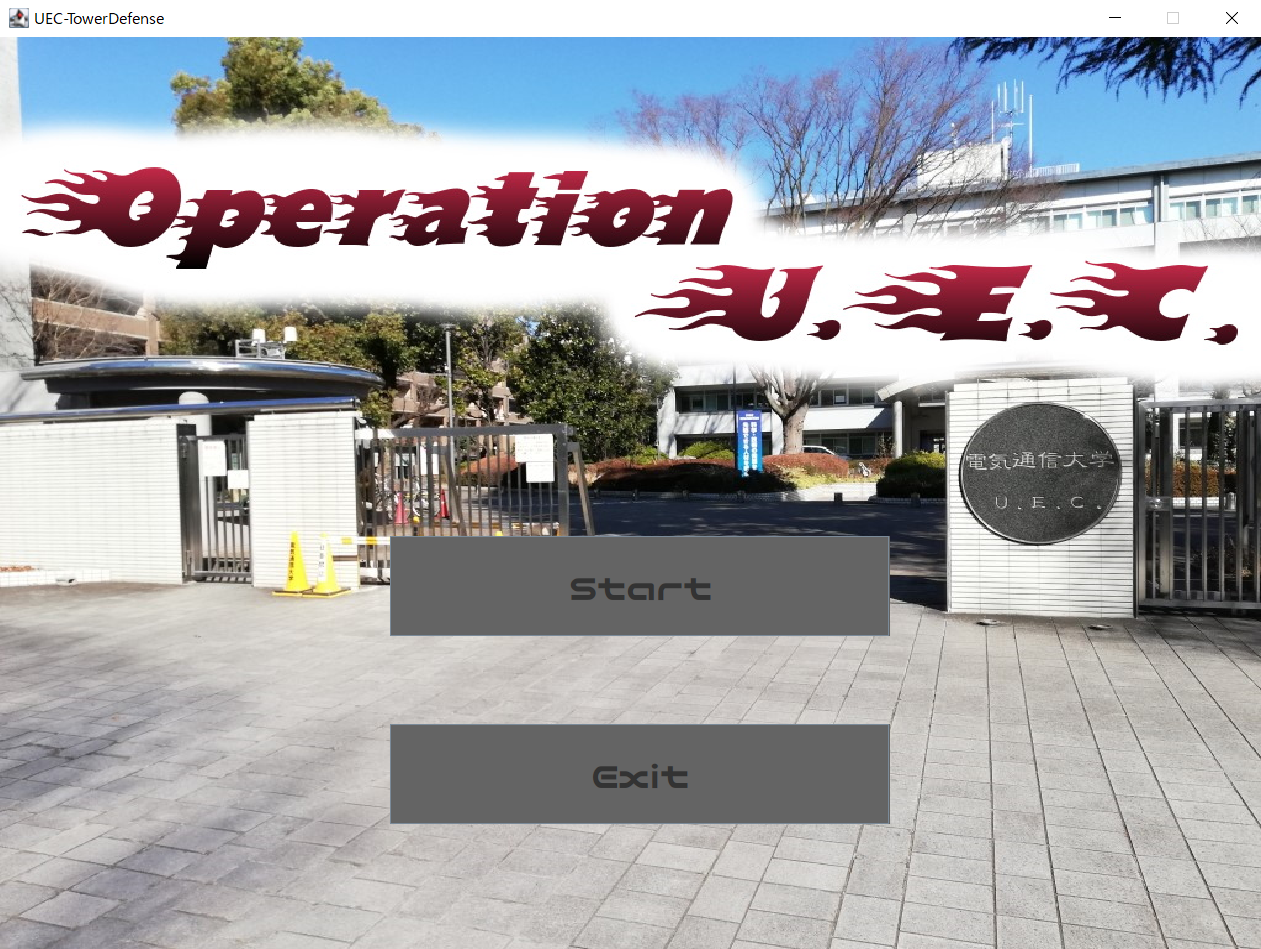
\includegraphics[width=0.6\textwidth]{title.png}
        \caption{タイトル画面。}
        \label{fig:title}
    \end{center}
\end{figure}

ゲームを開始すると、図\ref{fig:initscreen}の画面が表示される。画面上に所持金、防衛対象、ウェーブ開始までの残り時間が表示される。

\begin{figure}[H]
    \begin{center}
        \leavevmode
        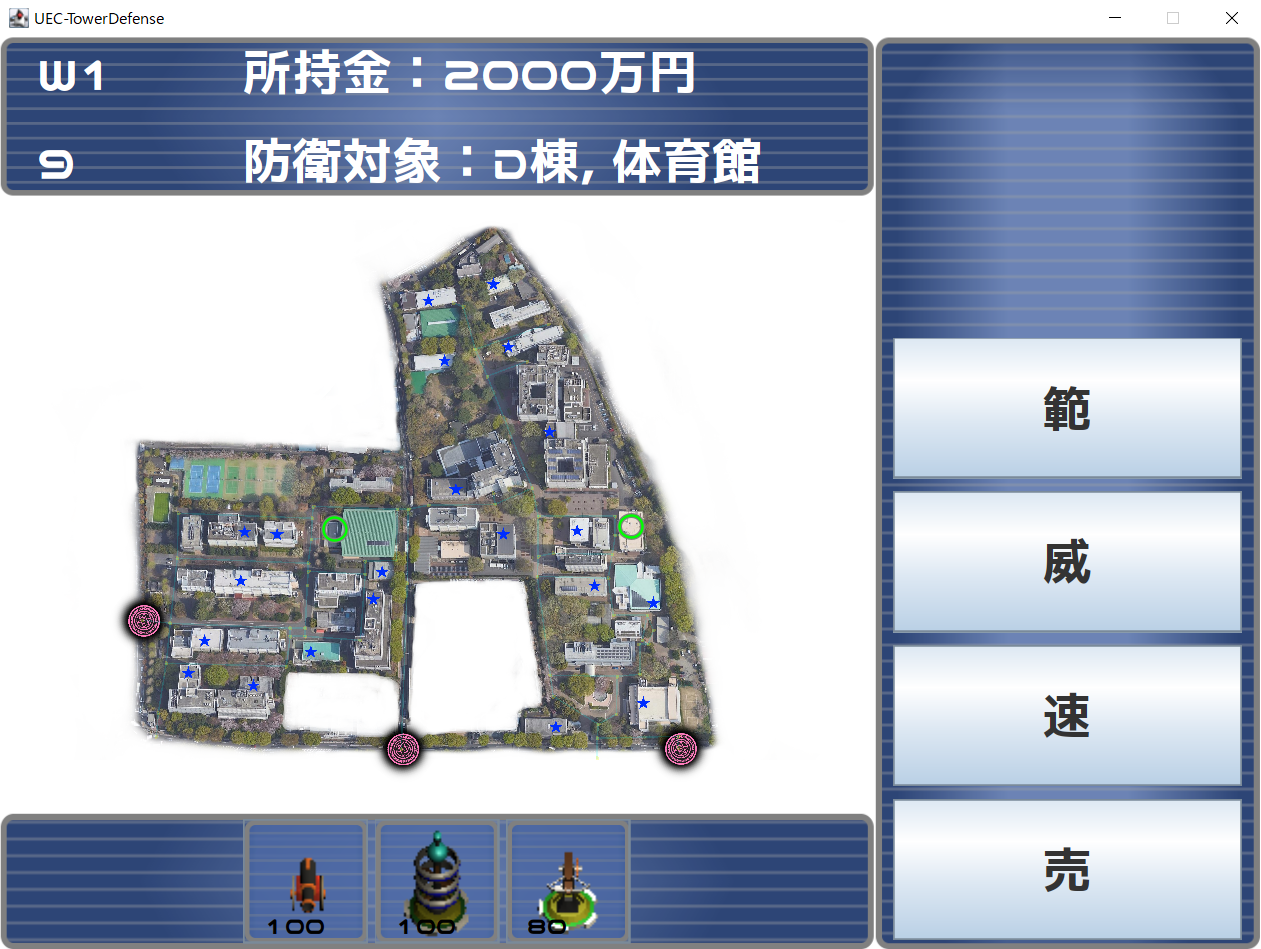
\includegraphics[width=0.6\textwidth]{initscreen.png}
        \caption{ゲームスタート直後の画面。}
        \label{fig:initscreen}
    \end{center}
\end{figure}

カメラ操作はシフトキーとスペースキーで拡縮を、W,A,S,Dキーで上下左右に移動することが出来る。図\ref{fig:zoomedscreen}に拡大したゲーム画面を示す。

\begin{figure}[H]
    \begin{center}
        \leavevmode
        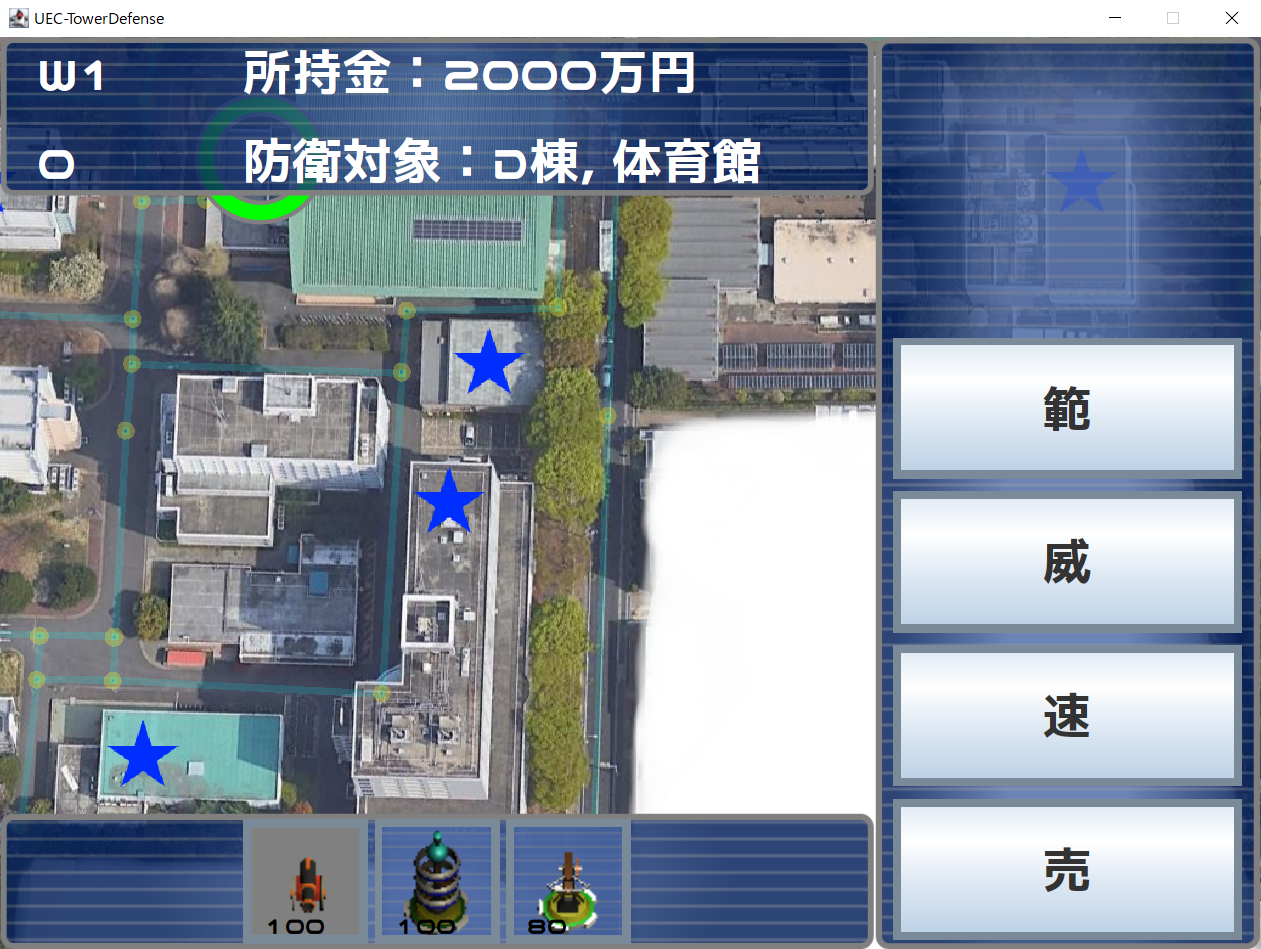
\includegraphics[width=0.6\textwidth]{zoomedscreen.png}
        \caption{シフトキーでゲームを画面ズームした状態。}
        \label{fig:zoomedscreen}
    \end{center}
\end{figure}

星形のアイコンがタレットを配置できる場所である。タレットを配置する際は、画面下のタレットのアイコンをクリックして選択し、マップ上の星形のアイコンをクリックすることで設置できる。図\ref{fig:turretplaced}に、マップ上にキャノンを配置した状態を示す。

\begin{figure}[H]
    \begin{center}
        \leavevmode
        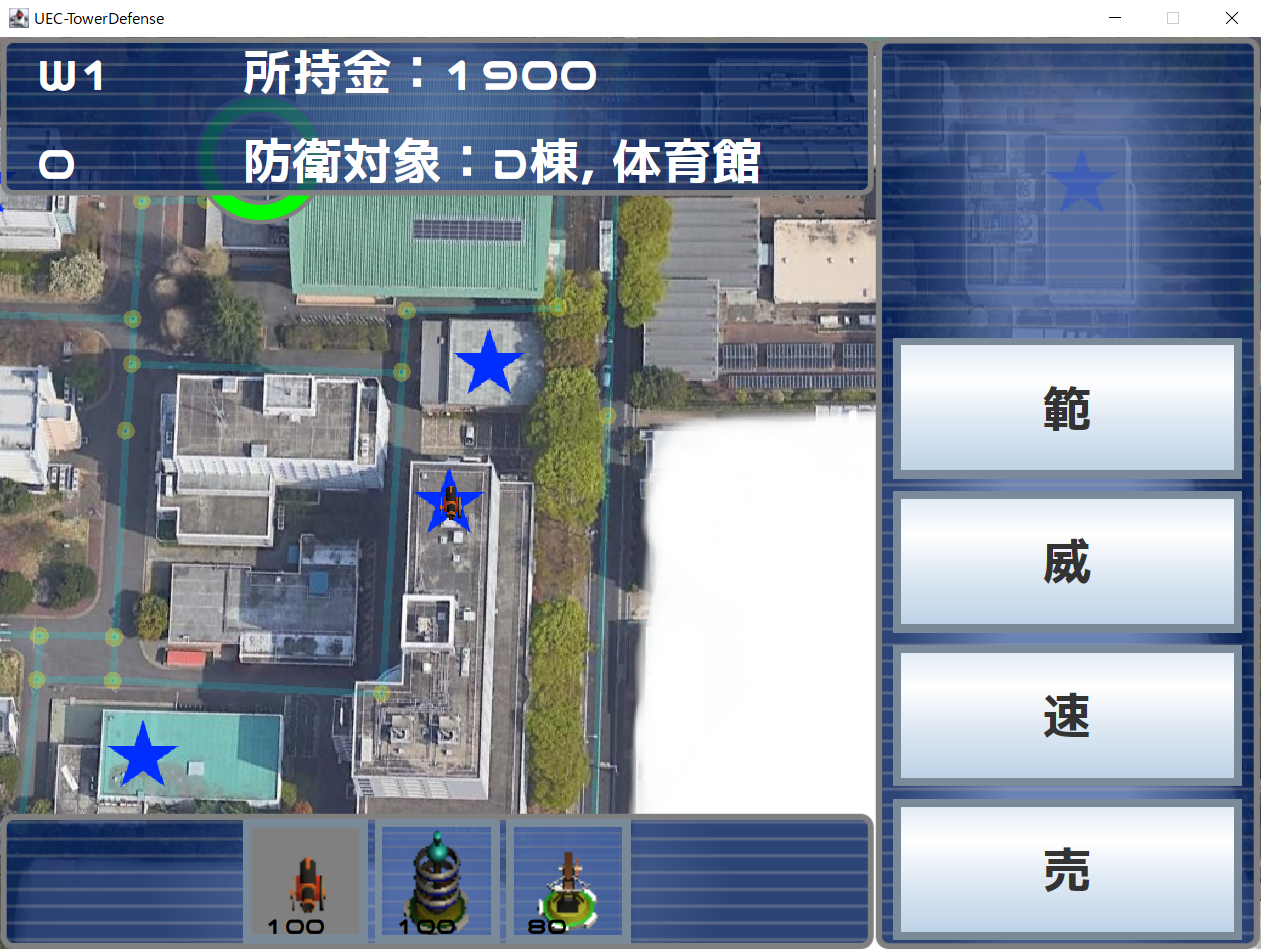
\includegraphics[width=0.6\textwidth]{turretplaced.png}
        \caption{キャノンを配置した状態。}
        \label{fig:turretplaced}
    \end{center}
\end{figure}

マップ上に配置したタレットを選択することで、敵を攻撃可能な範囲が赤い円で表示される。さらに、画面右にアップグレードと売却のメニューが表示される。タレットはキャノン、レーザー、バリスタの3種類あり、それぞれ特徴が異なる。一つ目のキャノンは攻撃範囲、威力、攻撃速度ともに平均的なタレットである。

\begin{figure}[H]
    \begin{center}
        \leavevmode
        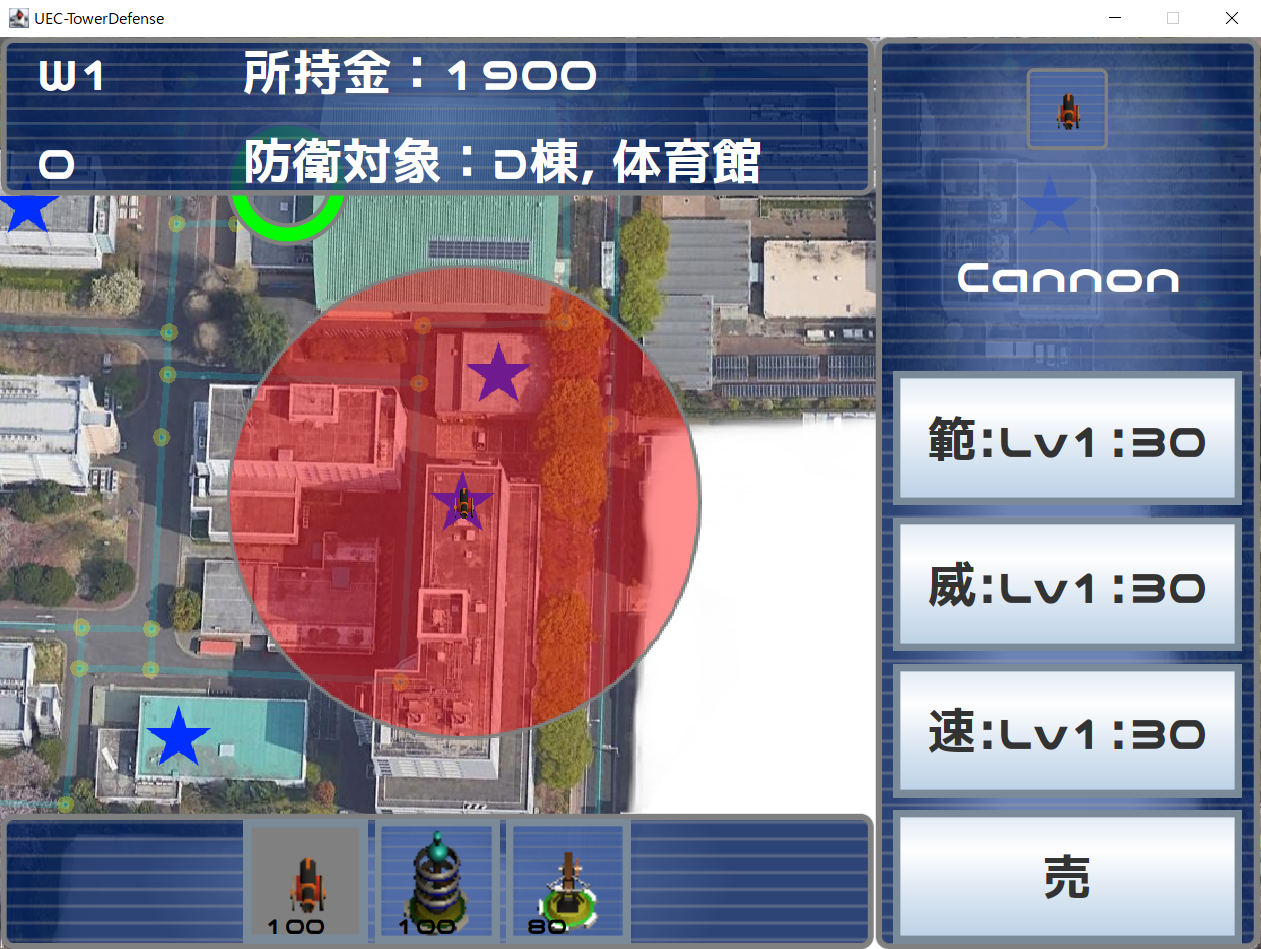
\includegraphics[width=0.6\textwidth]{turretrange.png}
        \caption{キャノンを選択した状態。}
        \label{fig:turretrange}
    \end{center}
\end{figure}

二つ目のレーザーは、攻撃範囲、威力ともに低いが、攻撃可能範囲内の全ての敵に対し継続してダメージを与えることができる。

\begin{figure}[H]
    \begin{center}
        \leavevmode
        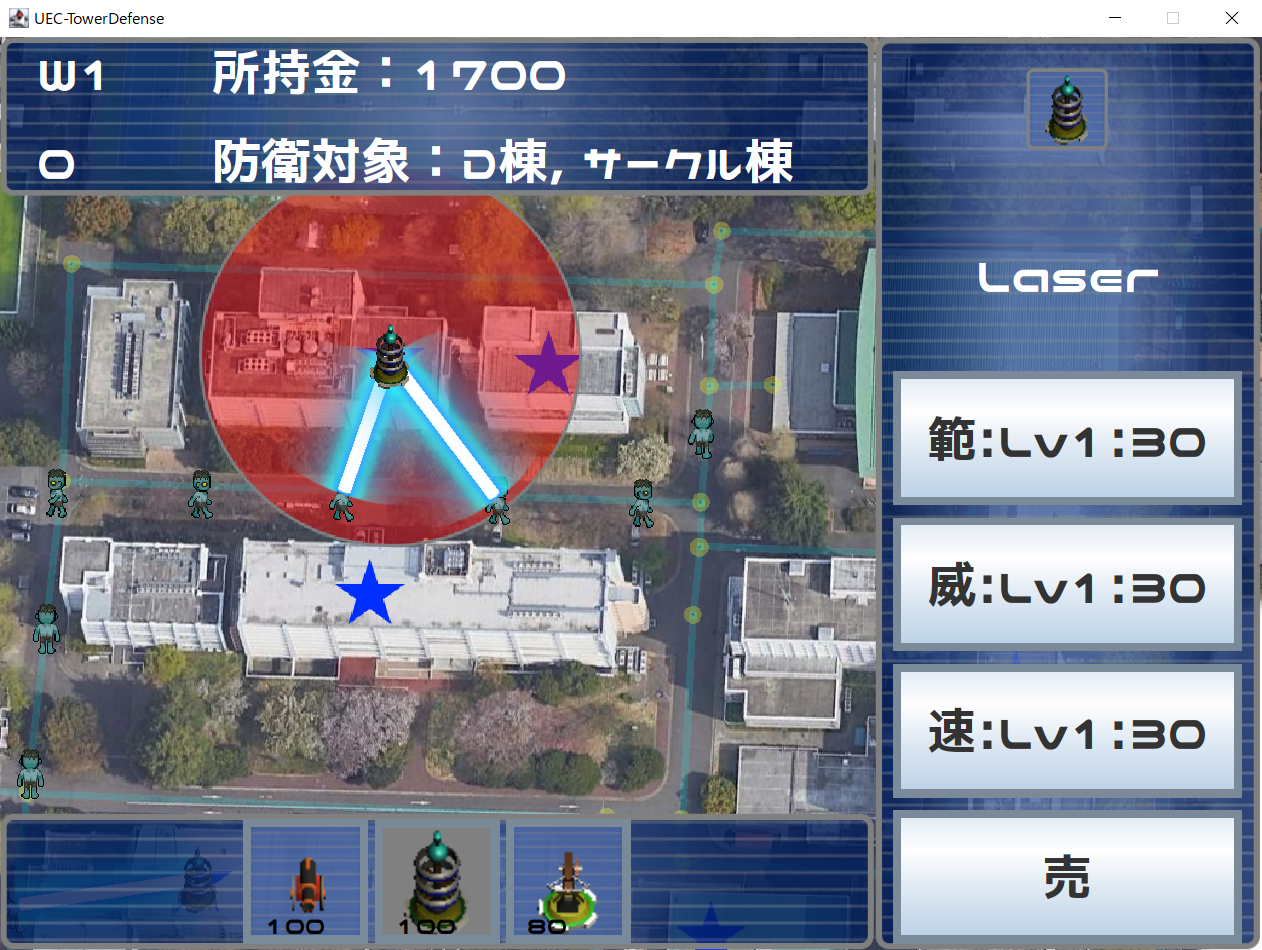
\includegraphics[width=0.6\textwidth]{laser.png}
        \caption{レーザーを配置した状態。範囲内の複数体の敵に同時に攻撃が可能。}
        \label{fig:laser}
    \end{center}
\end{figure}

三つ目のバリスタは、攻撃範囲、威力ともに高いが、攻撃速度が遅いタレットである。

\begin{figure}[H]
    \begin{center}
        \leavevmode
        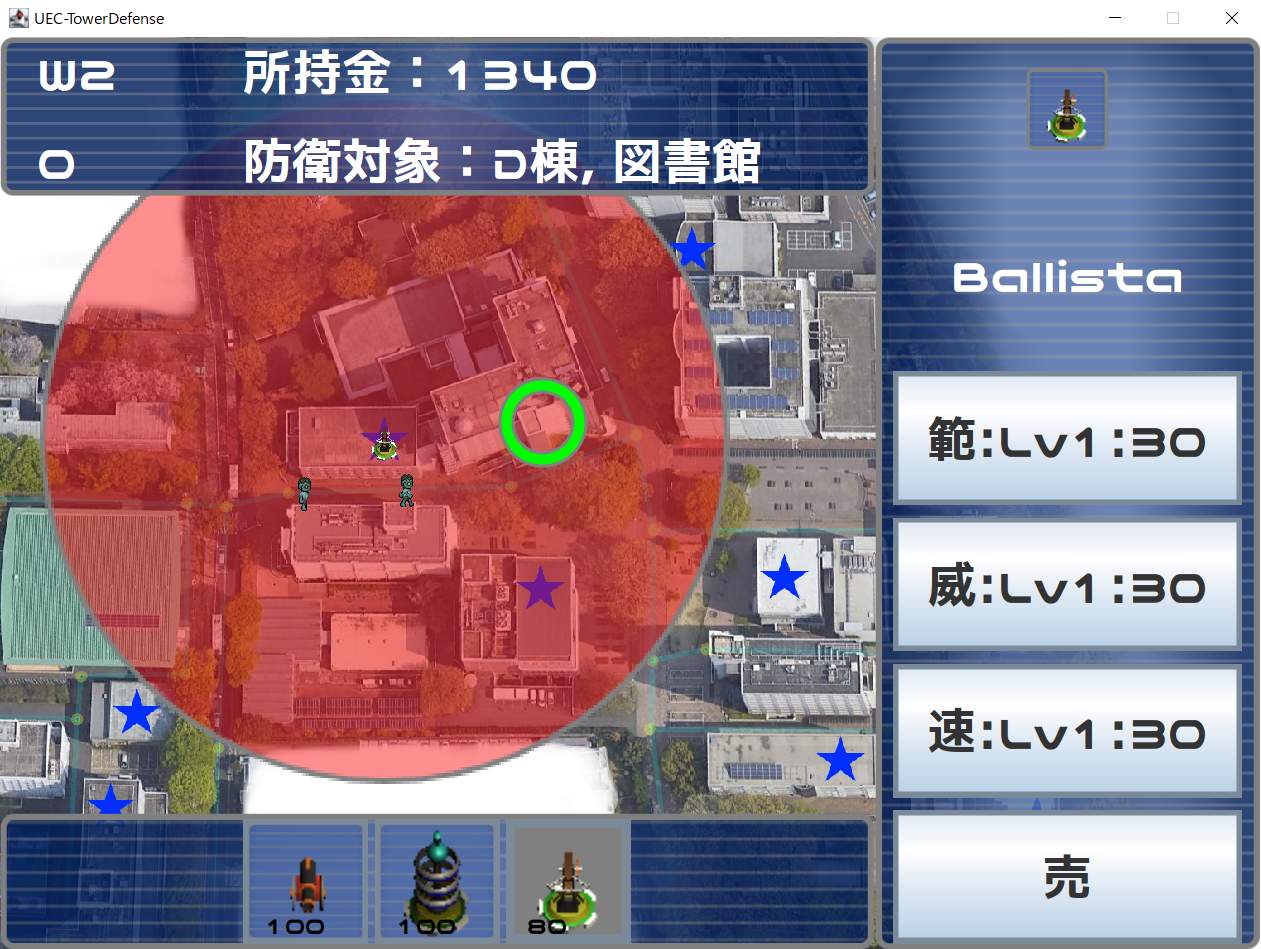
\includegraphics[width=0.6\textwidth]{ballista.png}
        \caption{バリスタを配置した状態。アップグレードをしていない状態でも攻撃範囲が広い。}
        \label{fig:ballista}
    \end{center}
\end{figure}

アップグレードの種類は攻撃範囲、威力、攻撃速度の3種類あり、アップグレードに対応するボタンを押すと一定の金額を消費して性能を強化することができる。アップグレードのレベルは10段階あり、タレット設置時は3種類ともレベル1である。画面右のアップグレードボタンには「アップグレードの種類:現在のレベル:消費する金額」が表示される。攻撃範囲のレベルを上げると、そのタレットが攻撃可能な半径が広がるため、赤い円の表示もそれに従って大きくなる。

\begin{figure}[H]
    \begin{center}
        \leavevmode
        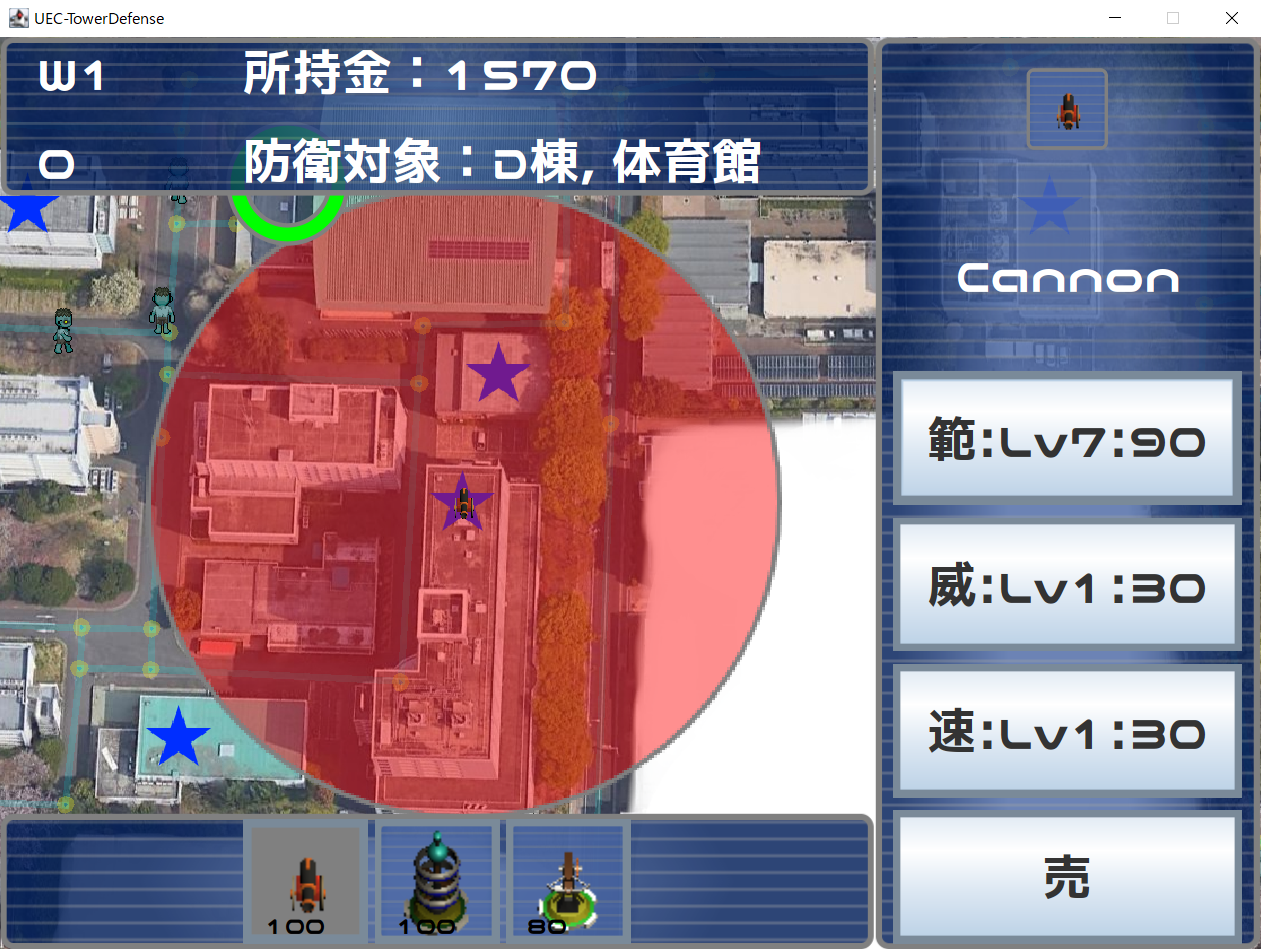
\includegraphics[width=0.6\textwidth]{rangeupgraded.png}
        \caption{攻撃範囲をレベル7まで強化した状態。図\ref{fig:turretrange}と比べると範囲が広くなっている。}
        \label{fig:rangeupgraded}
    \end{center}
\end{figure}

敵はマップ端の魔法陣から出現し、防衛対象に向かってくる。敵の種類はゾンビ、ゴブリン、ホブゴブリン、サイクロプスの4種類あり、以下のような特徴を持つ。

\begin{easylist}[itemize]
    @ ゾンビ
    @@ 体力、攻撃力、移動速度がいずれも平均的。
    @ ゴブリン
    @@ 体力と攻撃力は低いが、移動速度が速い。
    @ ホブゴブリン
    @@ 移動速度はゴブリンに劣るが、体力と攻撃力はゴブリンより強い。
    @ サイクロプス
    @@ 移動速度はかなり遅いが、体力と攻撃力が非常に高い。
\end{easylist}

敵を倒すと、敵ごとに一定の金額が手に入る。ウェーブを進めると、複数の魔法陣から敵が同時に出現したり、時間差で出現したりし難易度が上がる。複数種類の敵が同時に出現することもある。

\begin{figure}[H]
    \begin{center}
        \leavevmode
        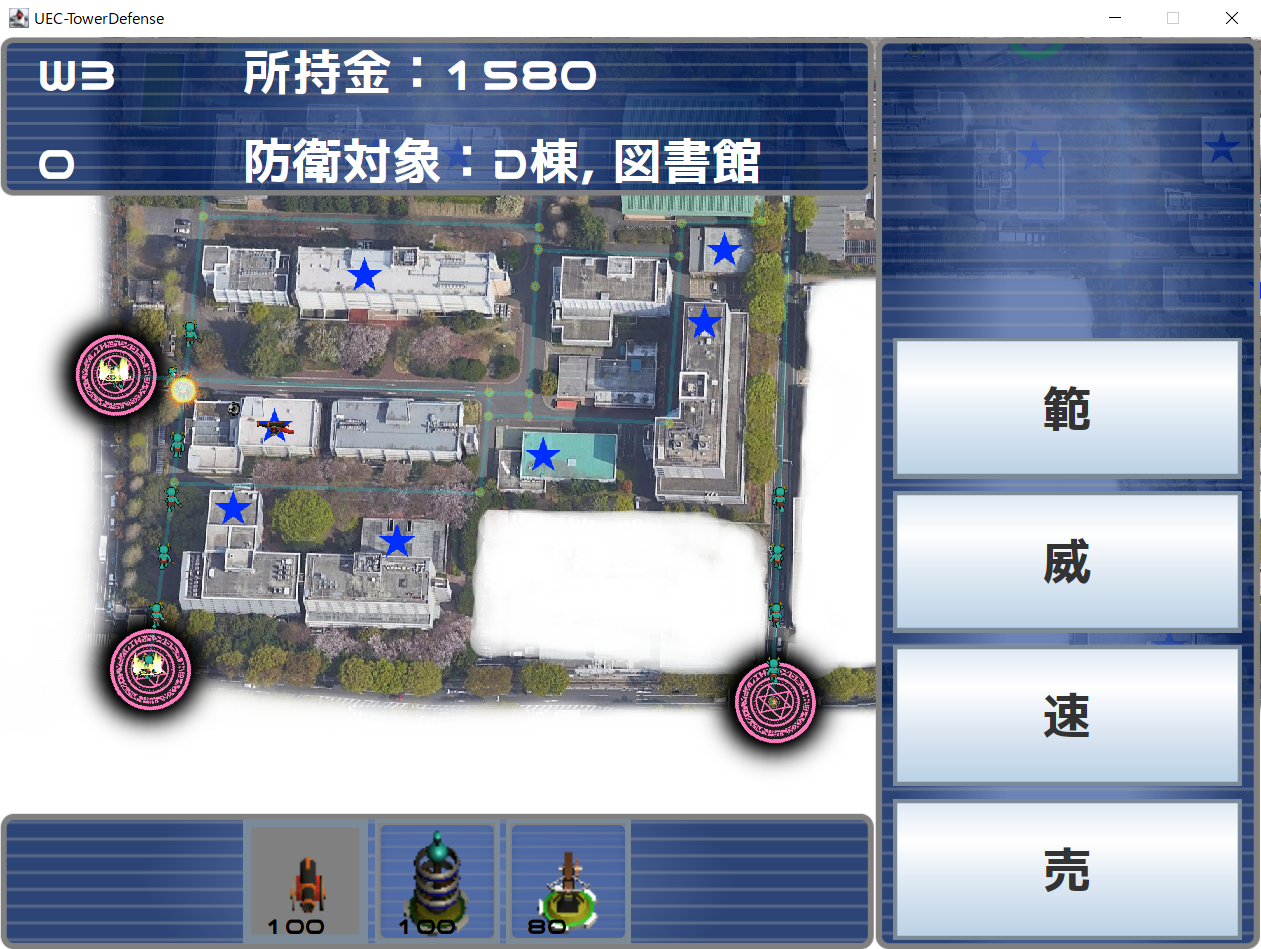
\includegraphics[width=0.6\textwidth]{multiplespawn.png}
        \caption{ウェーブが進むと、複数の魔法陣から敵が出現する。}
        \label{fig:multiplespawn}
    \end{center}
\end{figure}

防衛対象はゲーム開始時に候補地からランダムに2つ抽選で決定され、ゲーム開始直後は緑色の輪で表示される。この輪は、防衛対象の残りヒットポイントの表示としても機能しており、敵に攻撃されヒットポイントが減ると色が黄色、赤と変化する。

\begin{figure}[H]
    \begin{center}
        \leavevmode
        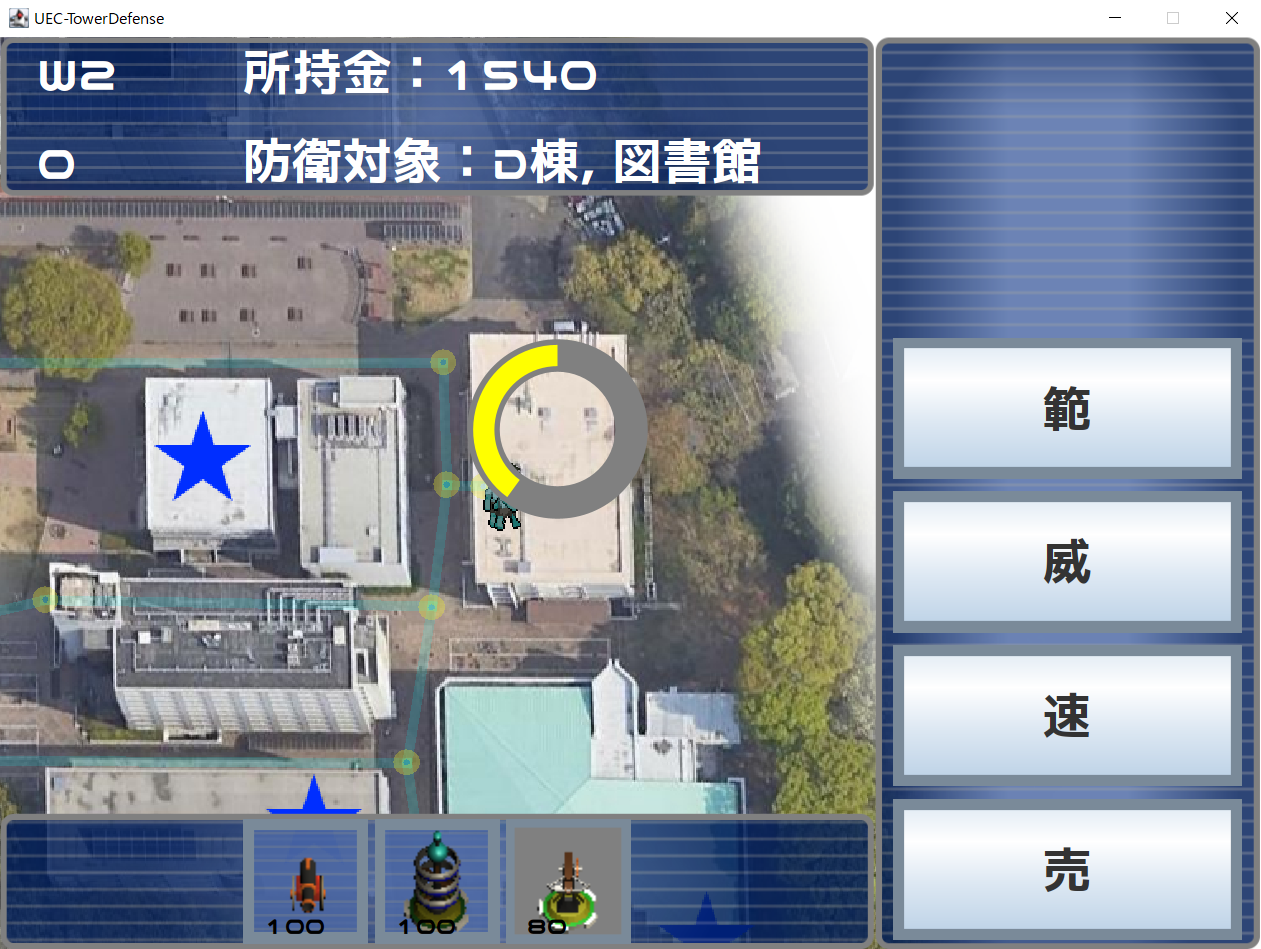
\includegraphics[width=0.6\textwidth]{beingattacked.png}
        \caption{防衛対象が攻撃を受けている状態。防衛対象のヒットポイントが減ると、輪の表示が変化する。}
        \label{fig:beingattacked}
    \end{center}
\end{figure}

防衛対象は、残りヒットポイントがゼロになると陥落する。

\begin{figure}[H]
    \begin{center}
        \leavevmode
        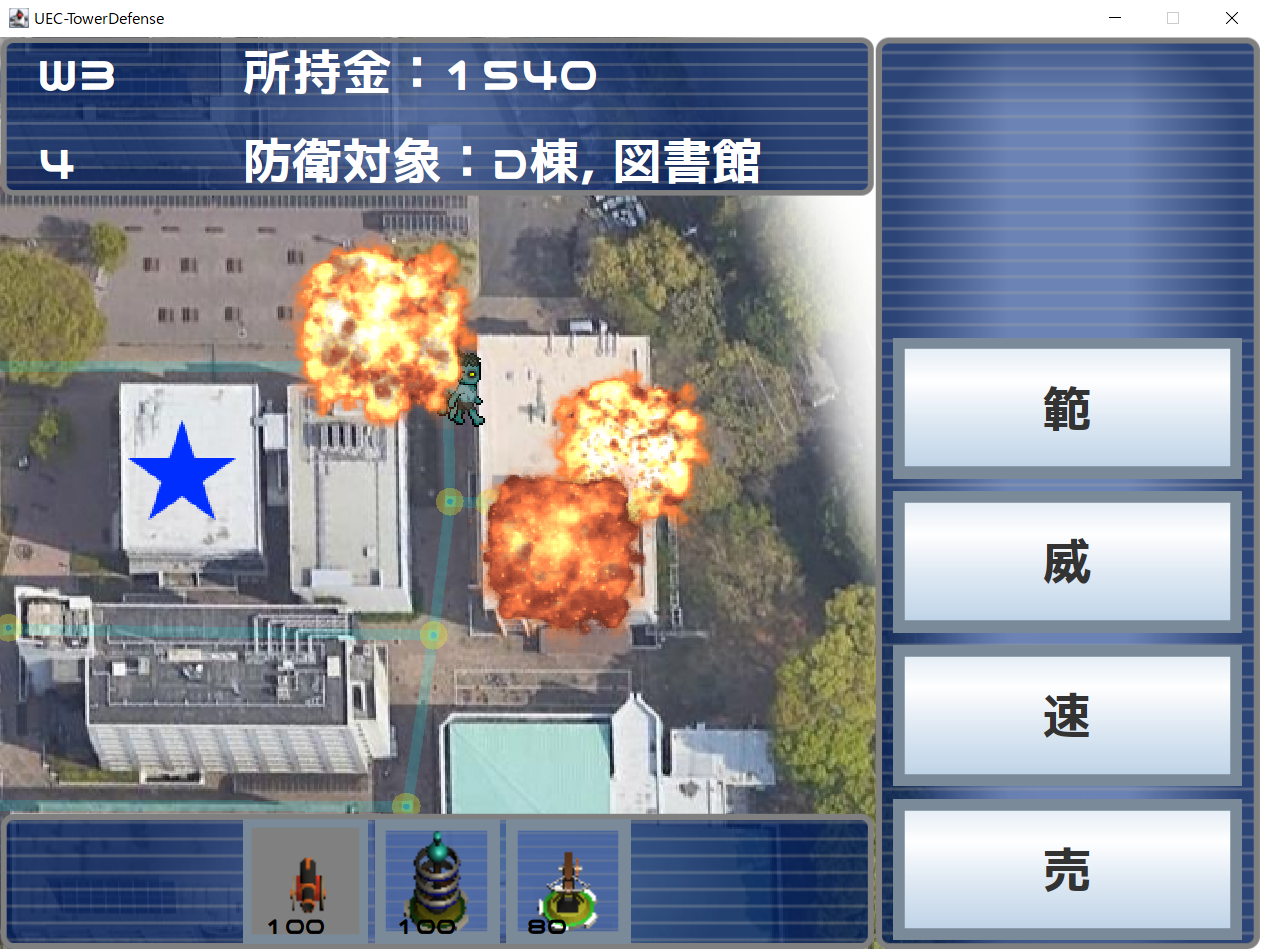
\includegraphics[width=0.6\textwidth]{destroyed.png}
        \caption{防衛対象が陥落した状態。}
        \label{fig:destroyed}
    \end{center}
\end{figure}

マップ上の全て、すなわち2つの防衛対象が陥落するとゲームオーバーとなる。

\begin{figure}[H]
    \begin{center}
        \leavevmode
        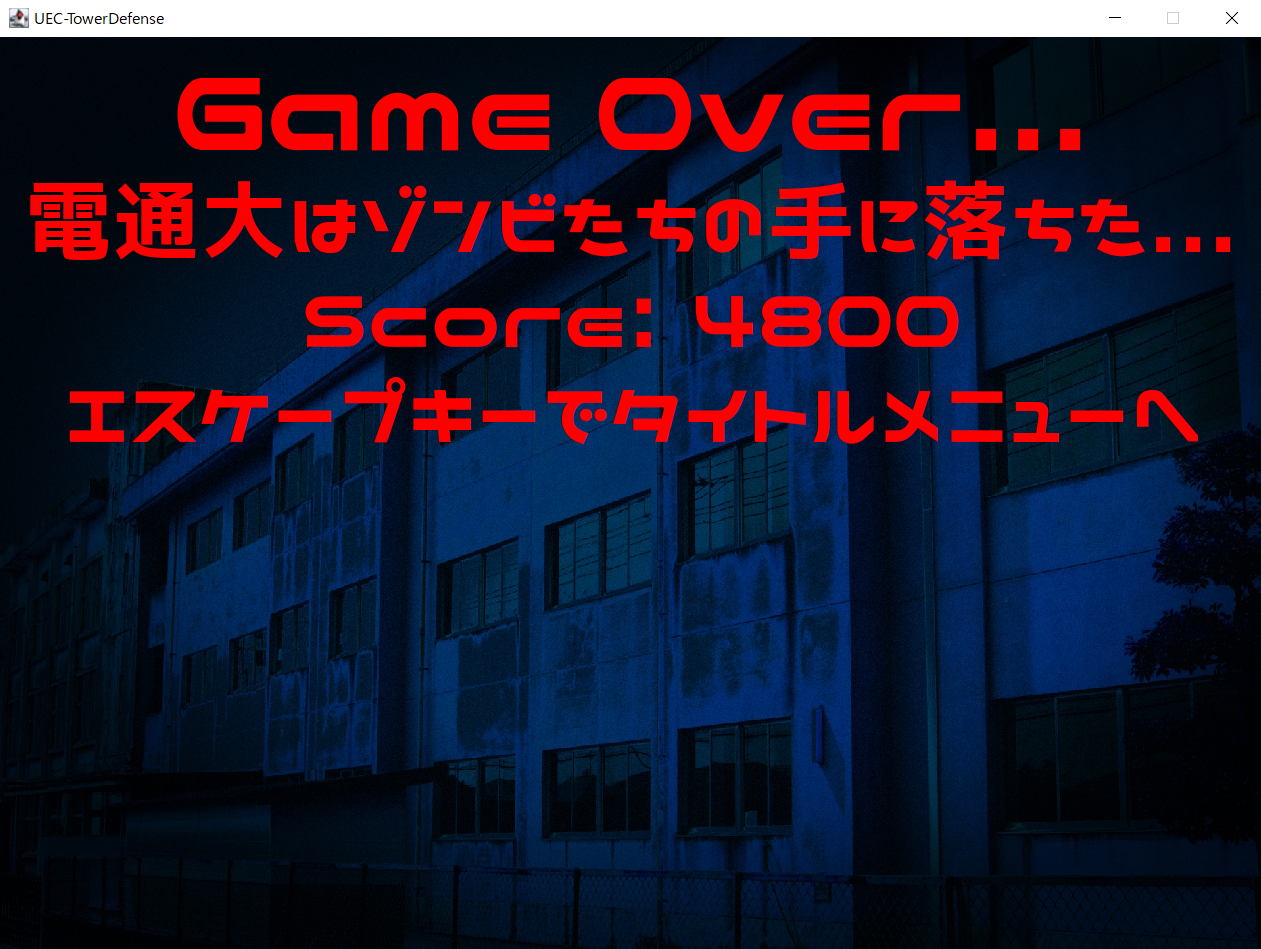
\includegraphics[width=0.6\textwidth]{gameover.png}
        \caption{ゲームオーバーのリザルト画面。}
        \label{fig:gameover}
    \end{center}
\end{figure}

一定のウェーブ数を凌ぎ切ると、ゲームクリアとなる。

\begin{figure}[H]
    \begin{center}
        \leavevmode
        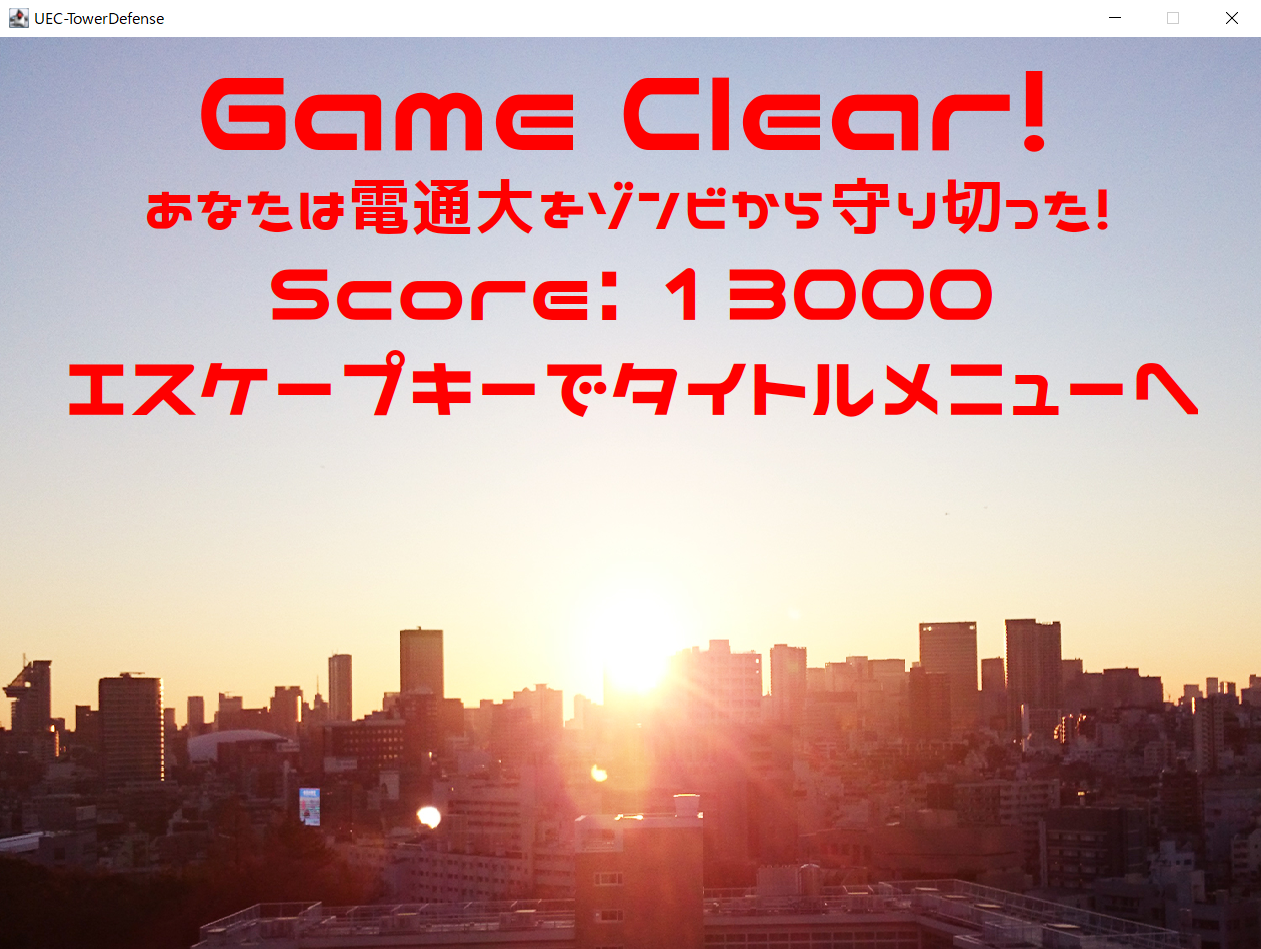
\includegraphics[width=0.6\textwidth]{gameclear.png}
        \caption{ゲームクリアのリザルト画面。}
        \label{fig:gameclear}
    \end{center}
\end{figure}

敵を倒すと、敵ごとに一定のスコアが得られる。リザルトに表示されるスコアは、ゲームオーバーの場合は敵の討伐時のスコアのみとなるが、ゲームクリアの場合は陥落していないタワーの数だけ一定のスコアがさらに加算される。

(文責: 上田)

\section{考察}

\subsection{プログラム制作の過程について}

制作するものを決定した直後の段階で細かい仕様を決定せず、初めにゲームシステムを作成し、次に必要となるクラスや機能を話し合っては実装を繰り返し、タレットや敵クラス、ゲームの進行の処理などを順に作成して完成に至った。

制作の過程では、自分が担当する機能やクラスを決定しても、その箇所をどう実装したら良いかわからず作業が頻繁に滞ることが大きな問題となった。具体的には、ゲームシステム部で定義されているクラスの役割がわからず適切な処理を記述できなかったり、細かい仕様が決定されておらず自分の担当箇所についての相談を頻繁に挟むということが生じた。原因は、ゲームシステムに関する知識の不足と、実装段階で仕様決定が不十分だったことにあると分析する。ゲームシステムでどのような機能が実装されているかが周知されていれば、自分でライブラリを探して実装するべきなのか否かが各々で判断できよりスムーズに開発ができたかもしれない。また、細かい仕様や分担を最初に決定したうえで実装をできていれば、毎回話し合う必要は無くなるだろう。しかし、プロジェクト自体が膨大であることや知識の差があったことを考慮すると、最初に隅々まで仕様を決めたうえで各自がコーディングする形で開発をするのは困難であったと推測する。

\subsection{完成したプログラムについて}

\begin{easylist}[itemize]
    @ MVCパターンを利用して各担当者で分業してそれぞれのコーディングを行う
    @ Modelの規模が大きいため、ゲームに登場する各オブジェクトを、Modelのことや他の担当者の担当範囲のことをほぼ知らなくてもよい粒度で分割して実装する
\end{easylist}
という当初の目的は達成できたと考える。しかし、各オブジェクトを独立して動作させるため情報の流れが複雑になってしまった結果、各オブジェクトが持っていなければならない情報を設計段階で見落としていると修正箇所がいくつかの場所にわたるといったこともあった。また、オブジェクトの生成が冗長になってしまった箇所がいくつか生じた。例えば、EnemySpawnerのコンストラクタは次のようになっている。

\begin{lstlisting}[numbers=none]
public EnemySpawner(GameObject root, GameObject parent, int initialDelay, int spawnDelay, int spawnCount, BaseEnemy spawnEnemy, Vertex initialVertex, EnemyParent enemyParent, EnemyDieListener enemyDieListener) {
    super(root, parent);
    this.initialDelay = initialDelay;
    this.spawnDelay = spawnDelay;
    this.spawnCount = spawnCount;
    this.spawnEnemy = spawnEnemy;
    this.initialVertex = initialVertex;
    this.enemyParent = enemyParent;
    this.enemyDieListener = enemyDieListener;
}
\end{lstlisting}

このような箇所に関しては、生成に関するデザインパターンの適用を考えるべきかもしれない。ゲームオブジェクトをマップ上に配置するためにはaddChild()を実行し、配置するゲームオブジェクトをゲームオブジェクトの木構造のヒエラルキーに入れる必要がある。addChildメソッドで、親にあたるゲームオブジェクトを自動的にオブジェクトに渡すことができれば、コンストラクタで親と根のゲームオブジェクトを渡さずに済み、冗長さをなくすことで情報の流れの見通しを改善できると考える。さらに、この設計では、オブジェクトの生成ごとに根と親を渡すため、誤った参照を渡すと木構造が破綻してしまう危険がある。システム部に関連する処理のバグをシステム部に関係ない場所で発生させてしまうという特定が困難なバグにつながりかねないため、その部分をシステム部以外には隠すような設計にするべきだったと考える。

一方で、システム部と各シーンの部分を分離したことで前のシーンなどに関係なく、各シーンに固有のことのみ考えてコーディングを行うことができた。これによって、シーン内の記述の簡潔さを保つともに、シーンごとの独立性も高くなるように設計することができた。また、エネミーの出現の実装では、Strategyパターンを用いることで、柔軟に出現アルゴリズムを変えるよう設計できた。

(文責: 上田)

\section{各自の反省と感想}
以下のような内容に関して,
メンバ全員がそれぞれ書いてください.メンバ間で
内容が重複しても構いません.必ず,それぞれ誰の
感想か分かるようにしてください.

\subsection{青木}

グループでのゲーム作成を通して、プログラミングを分業して行うことの難しさを学んだ。自身の担当クラスを書く為に、他のメンバーが書いたクラスを読み解くのが非常に大変だった。また、メンバー間でのjavaに関する知識の差が大きく、自分の担当クラスを書く時も他のメンバーから教わりながら作業を進めた為に、一部完全に分業が出来なかったクラスもあった。一方で、プログラムの統合に用いたGitHubを活用することで、クラスやフィールド、メソッドの名前の共有が非常にやりやすかった。

自身が担当したControllerクラスでは、キーボードとマウスによる操作を前提とした実装にしたが、タッチパネルによる操作が可能になれば操作性が非常に良くなるだろう。また、タレットを3種類作成したが、ゲームの設計段階では、エネミーの進行を阻む壁やエネミーの経路に設置できる地雷、さらには空を飛ぶエネミーに対して有効な対空砲などのタレットも案として挙がっていた。しかし、これらのタレットは設計難易度が高く、プログラムがうまく書けなかったので実装を断念した。いずれはこれらの機能を実装してゲーム性をさらに広げてみたいと思う。

Javaに関しては、オブジェクト指向で言語が構築されている分、応用性が非常に高い言語であると感じた。一方で、ゲーム制作などの特定の用途で用いる際には、ゲーム制作に特化しているUnityと比べて活用できる機能が少なく、不便に感じることが多々あった。また、MVCモデルによるプログラミングは、分業がしやすくなる分、MVCの分類を意識しながらコードを書くことが煩わしくなることが多かった。メンバーの持つ知識の差が少なく、完全に分業が出来た時にMVCモデルのありがたみを実感できるかもしれない。

プログラミング演習の授業に関して、初めて触れた高級言語であるjavaを短期間で効率良く学習することが出来たと思う。一方で、ゲーム作成の時に生かせる知識(各デザインパターンや木構造・グラフに関するライブラリの使い方など)を授業で触れることが出来れば、ゲーム制作がよりスムーズに進みそうだと感じた。

初めての高級言語によるプログラミングやゲーム制作を通して学ぶことが多くあった授業だった。

\subsection{上田}

ゲーム制作をするのは初めてで、シーン遷移やゲームシステムについて全く知識が無い状態であった。序盤は担当の箇所についてどう処理すれば良いかわからず、知識共有をしながらの作業がほとんどになってしまったが、最終的にはゲームシステムをある程度理解したうえでコーディングが出来るようになった。オブジェクト指向のプログラミングに慣れることができ、デザインパターンを使うメリットやクラス管理について理解を深めることが出来たと感じる。本講義を通しては、Javaやオブジェクト指向、デザインパターン、MVCモデルを学んだうえで実践でき、実際にアプリケーションを作成する力が身に付けることができた。プレゼンテーションでは、優秀賞を狙う意欲のあるグループが多かったように感じる。授業の内容だけでなく、各グループが制作したいものについて知識が深まったと考える。

完成したプログラムについては、タワーディフェンスとしては十分な機能を実装できたので、おおむね当初予定していた通りのものができたと考える。しかし、ゲーム内容としては一定のウェーブを凌ぎ切ればクリアというだけであり、ゲームとしてのやりこみ要素はまだ乏しい。ゲームの進行によりアイテムやポイントをためることで次回プレイで有利に進められるような要素を追加することで改善をできたらと思う。また、プレゼンテーションの際に受けた指摘でもあるが、画面外の敵の存在がわかるような表示ができるとより快適にプレイできると考える。

\subsubsection{青木}

グループでのゲーム作成を通して、プログラミングを分業して行うことの難しさを学んだ。自身の担当クラスを書く為に、他のメンバーが書いたクラスを読み解くのが非常に大変だった。また、メンバー間でのjavaに関する知識の差が大きく、自分の担当クラスを書く時も他のメンバーから教わりながら作業を進めた為に、一部完全に分業が出来なかったクラスもあった。一方で、プログラムの統合に用いたGitHubを活用することで、クラスやフィールド、メソッドの名前の共有が非常にやりやすかった。

自身が担当したControllerクラスでは、キーボードとマウスによる操作を前提とした実装にしたが、タッチパネルによる操作が可能になれば操作性が非常に良くなるだろう。また、タレットを3種類作成したが、ゲームの設計段階では、エネミーの進行を阻む壁やエネミーの経路に設置できる地雷、さらには空を飛ぶエネミーに対して有効な対空砲などのタレットも案として挙がっていた。しかし、これらのタレットは設計難易度が高く、プログラムがうまく書けなかったので実装を断念した。いずれはこれらの機能を実装してゲーム性をさらに広げてみたいと思う。

Javaに関しては、オブジェクト指向で言語が構築されている分、応用性が非常に高い言語であると感じた。一方で、ゲーム制作などの特定の用途で用いる際には、ゲーム制作に特化しているUnityと比べて活用できる機能が少なく、不便に感じることが多々あった。また、MVCモデルによるプログラミングは、分業がしやすくなる分、MVCの分類を意識しながらコードを書くことが煩わしくなることが多かった。メンバーの持つ知識の差が少なく、完全に分業が出来た時にMVCモデルのありがたみを実感できるかもしれない。

プログラミング演習の授業に関して、初めて触れた高級言語であるjavaを短期間で効率良く学習することが出来たと思う。一方で、ゲーム作成の時に生かせる知識(各デザインパターンや木構造・グラフに関するライブラリの使い方など)を授業で触れることが出来れば、ゲーム制作がよりスムーズに進みそうだと感じた。

初めての高級言語によるプログラミングやゲーム制作を通して学ぶことが多くあった授業だった。



\begin{itemize}
    \item グループでの作業を通しての反省や感想,それから考察できること.
    \item 今後の各自の担当部分の課題.やり残したこと.
    \item Javaやオブジェクト指向,MVCモデルなど学習内容に関する感想.
    \item 「プログラミング演習」の授業に関する感想や要望.
\end{itemize}

\newpage
\section*{付録1:操作法マニュアル (ユーザーズマニュアル)}
% そのプログラムを初めて使う人向けの説明書を書いてください.
% ドローエディタなら操作法の説明,ゲームならキー操作の
% 説明などを書いてください.スクリーンキャプチャした画像に
% 説明を書き込んだりしてもいいでしょう.
% 2ページ程度の簡潔な説明書で構いません.

% なお,付録は始まる直前で必ず改ページして下さい.

\begin{figure}[H]
    \centering
    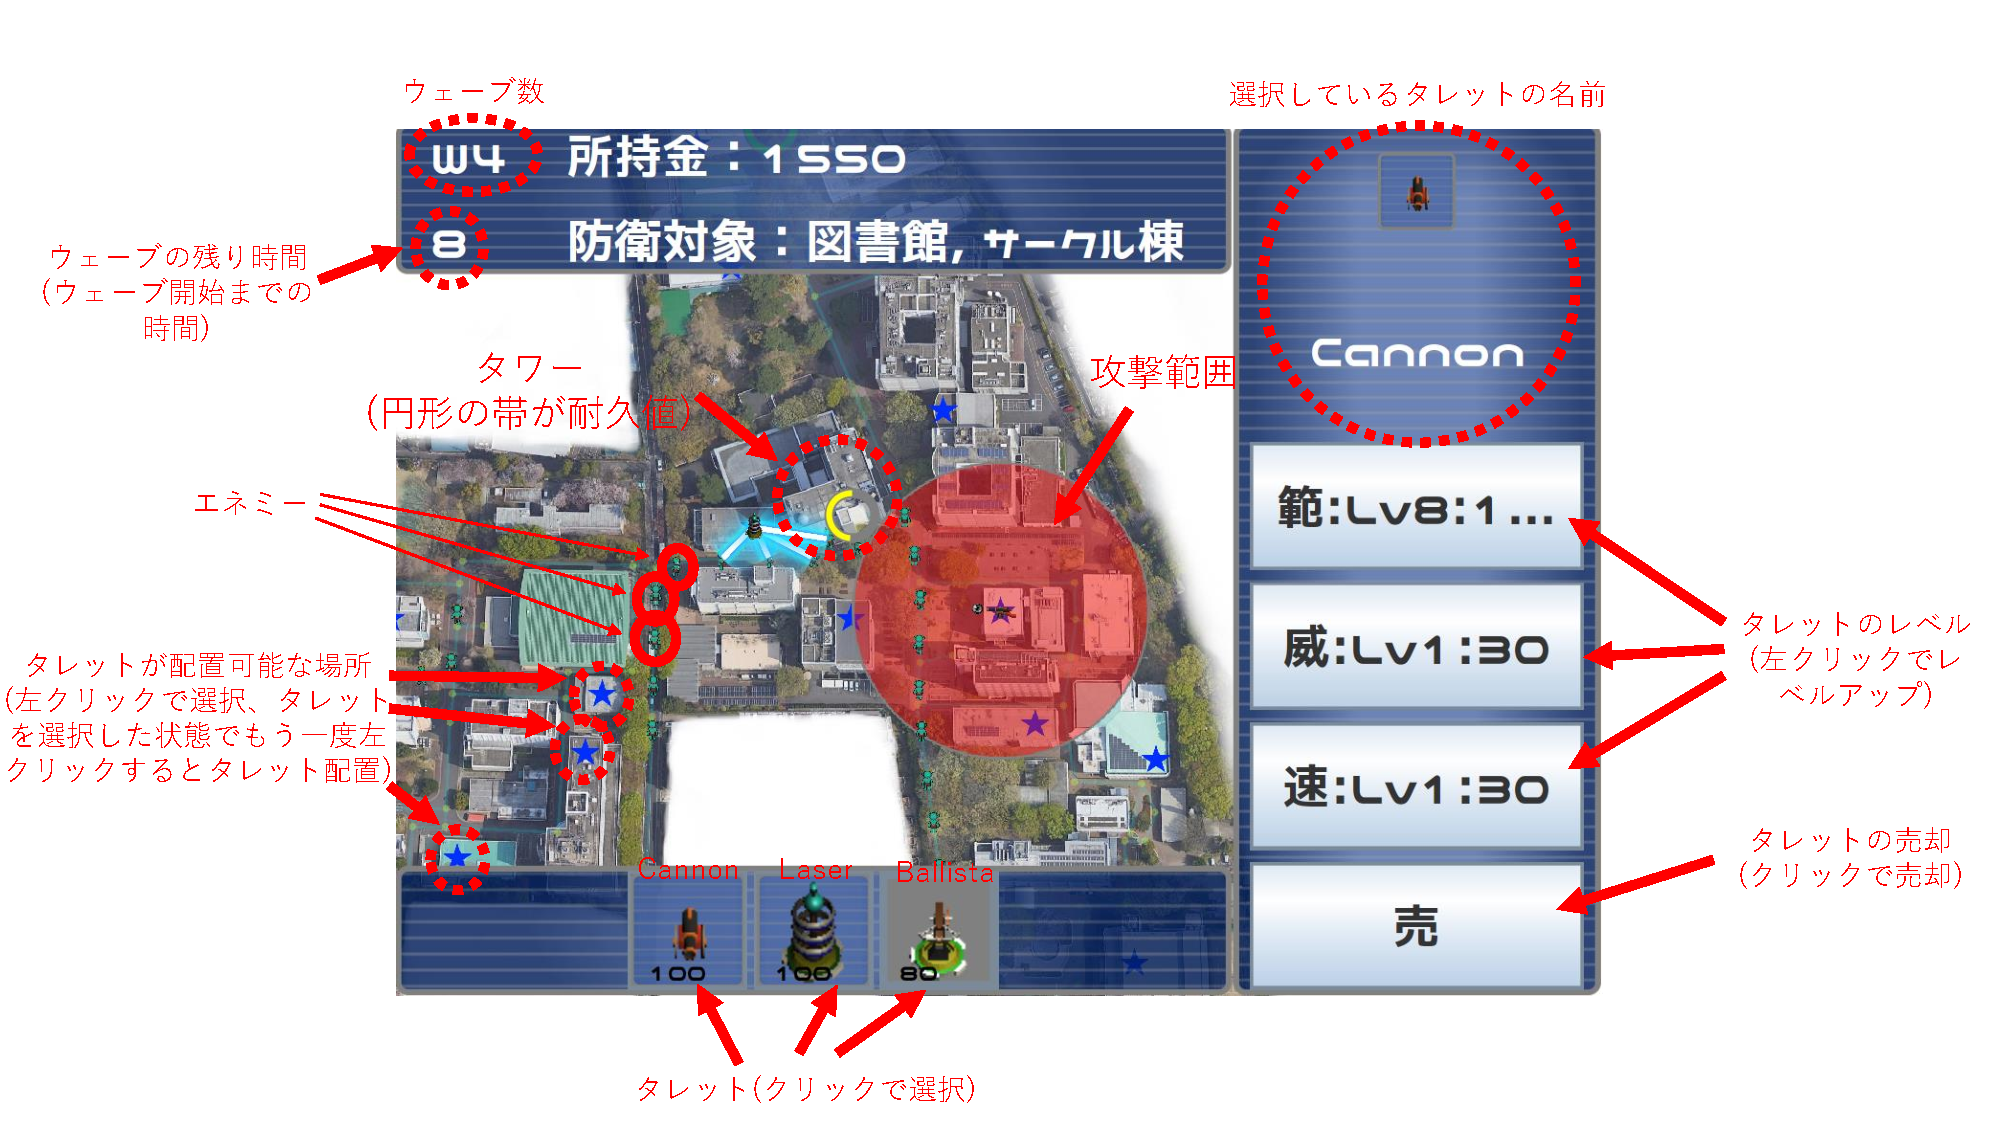
\includegraphics[width=0.95\textwidth, page=1]{manual.pdf}
    % \caption{Sample p.1}
    \label{Manual p.1}
\end{figure}

\begin{figure}[H]
    \centering
    \includegraphics[width=0.95\textwidth, page=2]{manual.pdf}
    % \caption{Manual p.2}
    \label{Manual p.2}
\end{figure}

\newpage
\section*{付録2:プログラムリスト}
% プログラムリストは本文中には説明に必要な部分だけ抜粋して掲載して,
% プログラムリスト全体はレポートの最後に「付録」として付ける.
% プログラムコードには,主なメソッド,フィールドの説明など
% 最低限のコメントは付ける.

% \lstinputlisting[caption=uectd.game.gameScene.Direction,label=Direction]{develop/uectd/game/gameScene/Direction.java}
% \lstinputlisting[caption=uectd.game.gameScene.gameMain.Arrow,label=Arrow]{develop/uectd/game/gameScene/gameMain/Arrow.java}
% \lstinputlisting[caption=uectd.game.gameScene.gameMain.BackGround,label=BackGround]{develop/uectd/game/gameScene/gameMain/BackGround.java}
% \lstinputlisting[caption=uectd.game.gameScene.gameMain.BallistaTurret,label=BallistaTurret]{develop/uectd/game/gameScene/gameMain/BallistaTurret.java}
% \lstinputlisting[caption=uectd.game.gameScene.gameMain.BaseEnemy,label=BaseEnemy]{develop/uectd/game/gameScene/gameMain/BaseEnemy.java}
% \lstinputlisting[caption=uectd.game.gameScene.gameMain.BaseEnemyActStrategy,label=BaseEnemyActStrategy]{develop/uectd/game/gameScene/gameMain/BaseEnemyActStrategy.java}
% \lstinputlisting[caption=uectd.game.gameScene.gameMain.BaseTurret,label=BaseTurret]{develop/uectd/game/gameScene/gameMain/BaseTurret.java}
% \lstinputlisting[caption=uectd.game.gameScene.gameMain.Cannonball,label=Cannonball]{develop/uectd/game/gameScene/gameMain/Cannonball.java}
% \lstinputlisting[caption=uectd.game.gameScene.gameMain.CannonTurret,label=CannonTurret]{develop/uectd/game/gameScene/gameMain/CannonTurret.java}
% \lstinputlisting[caption=uectd.game.gameScene.gameMain.Damage,label=Damage]{develop/uectd/game/gameScene/gameMain/Damage.java}
% \lstinputlisting[caption=uectd.game.gameScene.gameMain.enemy.Cyclopes,label=Cyclopes]{develop/uectd/game/gameScene/gameMain/enemy/Cyclopes.java}
% \lstinputlisting[caption=uectd.game.gameScene.gameMain.enemy.EnemyAnimation,label=EnemyAnimation]{develop/uectd/game/gameScene/gameMain/enemy/EnemyAnimation.java}
% \lstinputlisting[caption=uectd.game.gameScene.gameMain.enemy.Goblin,label=Goblin]{develop/uectd/game/gameScene/gameMain/enemy/Goblin.java}
% \lstinputlisting[caption=uectd.game.gameScene.gameMain.enemy.Hobgoblin,label=Hobgoblin]{develop/uectd/game/gameScene/gameMain/enemy/Hobgoblin.java}
% \lstinputlisting[caption=uectd.game.gameScene.gameMain.enemy.SearchAndDestroyStrategy,label=SearchAndDestroyStrategy]{develop/uectd/game/gameScene/gameMain/enemy/SearchAndDestroyStrategy.java}
% \lstinputlisting[caption=uectd.game.gameScene.gameMain.enemy.Zombie,label=Zombie]{develop/uectd/game/gameScene/gameMain/enemy/Zombie.java}
% \lstinputlisting[caption=uectd.game.gameScene.gameMain.EnemyDieEffect,label=EnemyDieEffect]{develop/uectd/game/gameScene/gameMain/EnemyDieEffect.java}
% \lstinputlisting[caption=uectd.game.gameScene.gameMain.EnemyDieListener,label=EnemyDieListener]{develop/uectd/game/gameScene/gameMain/EnemyDieListener.java}
% \lstinputlisting[caption=uectd.game.gameScene.gameMain.EnemyParent,label=EnemyParent]{develop/uectd/game/gameScene/gameMain/EnemyParent.java}
% \lstinputlisting[caption=uectd.game.gameScene.gameMain.EnemySpawner,label=EnemySpawner]{develop/uectd/game/gameScene/gameMain/EnemySpawner.java}
% \lstinputlisting[caption=uectd.game.gameScene.gameMain.EnemySpawnerArrangementStrategy,label=EnemySpawnerArrangementStrategy]{develop/uectd/game/gameScene/gameMain/EnemySpawnerArrangementStrategy.java}
% \lstinputlisting[caption=uectd.game.gameScene.gameMain.EnemySpawnerEffect,label=EnemySpawnerEffect]{develop/uectd/game/gameScene/gameMain/EnemySpawnerEffect.java}
% \lstinputlisting[caption=uectd.game.gameScene.gameMain.EnemySpawnerManager,label=EnemySpawnerManager]{develop/uectd/game/gameScene/gameMain/EnemySpawnerManager.java}
% \lstinputlisting[caption=uectd.game.gameScene.gameMain.EnemySpawnerMark,label=EnemySpawnerMark]{develop/uectd/game/gameScene/gameMain/EnemySpawnerMark.java}
% \lstinputlisting[caption=uectd.game.gameScene.gameMain.EnemySpawnerParent,label=EnemySpawnerParent]{develop/uectd/game/gameScene/gameMain/EnemySpawnerParent.java}
% \lstinputlisting[caption=uectd.game.gameScene.gameMain.FileReadSpawnStrategy,label=FileReadSpawnStrategy]{develop/uectd/game/gameScene/gameMain/FileReadSpawnStrategy.java}
% \lstinputlisting[caption=uectd.game.gameScene.gameMain.GameLevel,label=GameLevel]{develop/uectd/game/gameScene/gameMain/GameLevel.java}
% \lstinputlisting[caption=uectd.game.gameScene.gameMain.Graph,label=Graph]{develop/uectd/game/gameScene/gameMain/Graph.java}
% \lstinputlisting[caption=uectd.game.gameScene.gameMain.GraphBuilder,label=GraphBuilder]{develop/uectd/game/gameScene/gameMain/GraphBuilder.java}
% \lstinputlisting[caption=uectd.game.gameScene.gameMain.IAttackable,label=IAttackable]{develop/uectd/game/gameScene/gameMain/IAttackable.java}
% \lstinputlisting[caption=uectd.game.gameScene.gameMain.IDamageApplicable,label=IDamageApplicable]{develop/uectd/game/gameScene/gameMain/IDamageApplicable.java}
% \lstinputlisting[caption=uectd.game.gameScene.gameMain.IMoneyTransfer,label=IMoneyTransfer]{develop/uectd/game/gameScene/gameMain/IMoneyTransfer.java}
% \lstinputlisting[caption=uectd.game.gameScene.gameMain.Laser,label=Laser]{develop/uectd/game/gameScene/gameMain/Laser.java}
% \lstinputlisting[caption=uectd.game.gameScene.gameMain.LaserTurret,label=LaserTurret]{develop/uectd/game/gameScene/gameMain/LaserTurret.java}
% \lstinputlisting[caption=uectd.game.gameScene.gameMain.SearchEnemyField,label=SearchEnemyField]{develop/uectd/game/gameScene/gameMain/SearchEnemyField.java}
% \lstinputlisting[caption=uectd.game.gameScene.gameMain.Tower,label=Tower]{develop/uectd/game/gameScene/gameMain/Tower.java}
% \lstinputlisting[caption=uectd.game.gameScene.gameMain.TowerArranger,label=TowerArranger]{develop/uectd/game/gameScene/gameMain/TowerArranger.java}
% \lstinputlisting[caption=uectd.game.gameScene.gameMain.TowerFallEffect,label=TowerFallEffect]{develop/uectd/game/gameScene/gameMain/TowerFallEffect.java}
% \lstinputlisting[caption=uectd.game.gameScene.gameMain.TowerFallEffectSub,label=TowerFallEffectSub]{develop/uectd/game/gameScene/gameMain/TowerFallEffectSub.java}
% \lstinputlisting[caption=uectd.game.gameScene.gameMain.TowerFallListener,label=TowerFallListener]{develop/uectd/game/gameScene/gameMain/TowerFallListener.java}
% \lstinputlisting[caption=uectd.game.gameScene.gameMain.TowerParent,label=TowerParent]{develop/uectd/game/gameScene/gameMain/TowerParent.java}
% \lstinputlisting[caption=uectd.game.gameScene.gameMain.TurretAttackToEnemyEffect,label=TurretAttackToEnemyEffect]{develop/uectd/game/gameScene/gameMain/TurretAttackToEnemyEffect.java}
% \lstinputlisting[caption=uectd.game.gameScene.gameMain.TurretParent,label=TurretParent]{develop/uectd/game/gameScene/gameMain/TurretParent.java}
% \lstinputlisting[caption=uectd.game.gameScene.gameMain.TurretSocket,label=TurretSocket]{develop/uectd/game/gameScene/gameMain/TurretSocket.java}
% \lstinputlisting[caption=uectd.game.gameScene.gameMain.TurretSocketArranger,label=TurretSocketArranger]{develop/uectd/game/gameScene/gameMain/TurretSocketArranger.java}
% \lstinputlisting[caption=uectd.game.gameScene.gameMain.TurretSocketParent,label=TurretSocketParent]{develop/uectd/game/gameScene/gameMain/TurretSocketParent.java}
% \lstinputlisting[caption=uectd.game.gameScene.GameScene,label=GameScene]{develop/uectd/game/gameScene/GameScene.java}
% \lstinputlisting[caption=uectd.game.gameScene.GameSceneController,label=GameSceneController]{develop/uectd/game/gameScene/GameSceneController.java}
% \lstinputlisting[caption=uectd.game.gameScene.GameSceneModel,label=GameSceneModel]{develop/uectd/game/gameScene/GameSceneModel.java}
% \lstinputlisting[caption=uectd.game.gameScene.GameSceneView,label=GameSceneView]{develop/uectd/game/gameScene/GameSceneView.java}
% \lstinputlisting[caption=uectd.game.pauseScene.PauseScene,label=PauseScene]{develop/uectd/game/pauseScene/PauseScene.java}
% \lstinputlisting[caption=uectd.game.pauseScene.PauseSceneController,label=PauseSceneController]{develop/uectd/game/pauseScene/PauseSceneController.java}
% \lstinputlisting[caption=uectd.game.pauseScene.PauseSceneModel,label=PauseSceneModel]{develop/uectd/game/pauseScene/PauseSceneModel.java}
% \lstinputlisting[caption=uectd.game.pauseScene.PauseSceneView,label=PauseSceneView]{develop/uectd/game/pauseScene/PauseSceneView.java}
% \lstinputlisting[caption=uectd.game.ResourcePathDefines,label=ResourcePathDefines]{develop/uectd/game/ResourcePathDefines.java}
% \lstinputlisting[caption=uectd.game.resultScene.ResultScene,label=ResultScene]{develop/uectd/game/resultScene/ResultScene.java}
% \lstinputlisting[caption=uectd.game.resultScene.ResultSceneController,label=ResultSceneController]{develop/uectd/game/resultScene/ResultSceneController.java}
% \lstinputlisting[caption=uectd.game.resultScene.ResultSceneModel,label=ResultSceneModel]{develop/uectd/game/resultScene/ResultSceneModel.java}
% \lstinputlisting[caption=uectd.game.resultScene.ResultSceneView,label=ResultSceneView]{develop/uectd/game/resultScene/ResultSceneView.java}
% \lstinputlisting[caption=uectd.game.titleScene.TitleScene,label=TitleScene]{develop/uectd/game/titleScene/TitleScene.java}
% \lstinputlisting[caption=uectd.game.titleScene.TitleSceneController,label=TitleSceneController]{develop/uectd/game/titleScene/TitleSceneController.java}
% \lstinputlisting[caption=uectd.game.titleScene.TitleSceneModel,label=TitleSceneModel]{develop/uectd/game/titleScene/TitleSceneModel.java}
% \lstinputlisting[caption=uectd.game.titleScene.TitleSceneView,label=TitleSceneView]{develop/uectd/game/titleScene/TitleSceneView.java}
% \lstinputlisting[caption=uectd.gameSystem.Define,label=Define]{develop/uectd/gameSystem/Define.java}
% \lstinputlisting[caption=uectd.gameSystem.GameObject,label=GameObject]{develop/uectd/gameSystem/GameObject.java}
% \lstinputlisting[caption=uectd.gameSystem.MainFrame,label=MainFrame]{develop/uectd/gameSystem/MainFrame.java}
% \lstinputlisting[caption=uectd.gameSystem.Scene,label=Scene]{develop/uectd/gameSystem/Scene.java}
% \lstinputlisting[caption=uectd.gameSystem.SceneChangeListener,label=SceneChangeListener]{develop/uectd/gameSystem/SceneChangeListener.java}
% \lstinputlisting[caption=uectd.gameSystem.SceneController,label=SceneController]{develop/uectd/gameSystem/SceneController.java}
% \lstinputlisting[caption=uectd.gameSystem.SceneModel,label=SceneModel]{develop/uectd/gameSystem/SceneModel.java}
% \lstinputlisting[caption=uectd.gameSystem.SceneView,label=SceneView]{develop/uectd/gameSystem/SceneView.java}
% \lstinputlisting[caption=uectd.gameSystem.util.AnimationSprite,label=AnimationSprite]{develop/uectd/gameSystem/util/AnimationSprite.java}
% \lstinputlisting[caption=uectd.gameSystem.util.Camera,label=Camera]{develop/uectd/gameSystem/util/Camera.java}
% \lstinputlisting[caption=uectd.gameSystem.util.CircleCollider,label=CircleCollider]{develop/uectd/gameSystem/util/CircleCollider.java}
% \lstinputlisting[caption=uectd.gameSystem.util.Collider,label=Collider]{develop/uectd/gameSystem/util/Collider.java}
% \lstinputlisting[caption=uectd.gameSystem.util.Drawable,label=Drawable]{develop/uectd/gameSystem/util/Drawable.java}
% \lstinputlisting[caption=uectd.gameSystem.util.Effect,label=Effect]{develop/uectd/gameSystem/util/Effect.java}
% \lstinputlisting[caption=uectd.gameSystem.util.GameSound,label=GameSound]{develop/uectd/gameSystem/util/GameSound.java}
% \lstinputlisting[caption=uectd.gameSystem.util.GameTimer,label=GameTimer]{develop/uectd/gameSystem/util/GameTimer.java}
% \lstinputlisting[caption=uectd.gameSystem.util.IClickable,label=IClickable]{develop/uectd/gameSystem/util/IClickable.java}
% \lstinputlisting[caption=uectd.gameSystem.util.ImageManager,label=ImageManager]{develop/uectd/gameSystem/util/ImageManager.java}
% \lstinputlisting[caption=uectd.gameSystem.util.Intent,label=Intent]{develop/uectd/gameSystem/util/Intent.java}
% \lstinputlisting[caption=uectd.gameSystem.util.ObservableComponent,label=ObservableComponent]{develop/uectd/gameSystem/util/ObservableComponent.java}
% \lstinputlisting[caption=uectd.gameSystem.util.SoundManager,label=SoundManager]{develop/uectd/gameSystem/util/SoundManager.java}
% \lstinputlisting[caption=uectd.gameSystem.util.Sprite,label=Sprite]{develop/uectd/gameSystem/util/Sprite.java}
% \lstinputlisting[caption=uectd.gameSystem.util.Vector2,label=Vector2]{develop/uectd/gameSystem/util/Vector2.java}


% \ref{label} で参照

\end{document}